% called by main.tex
%
\chapter{Project development}
\label{ch::chapter5}

\section{Design, Pipeline and Overview}
This section will describe the general process of the project as shown in the image \ref{fig:Project-Diagram}. This image shows in broad outline the stages that have been developed in this project, focusing only on the procedures followed with the data provided by the University Hospital of Burgos (HUBU).

\begin{tcolorbox}
The dataset provided by HUBU has \textbf{63 video files} organised in different directories: Unclassified (58 files), Mild\_encephalopathy (1 file), Severe\_encephalopathy (1 file), Moderate\_encephalopathy (1 file), and No\_encephalopathy  (2 files).
\end{tcolorbox}


The first stage includes the decomposition of the HUBU videos, where audio was extracted from each file, and stored under the same name, but with a different extension. Then, each of the audio files was manually labelled. For the creation of these labels, a vector has been generated with a length equal to the number of seconds that each audio file. The vector is composed of \textbf{0’s} and \textbf{1’s} in which the former indicates \textbf{that the baby is crying} in that second of the audio, and the latter \textbf{that the baby is not crying}. This is regardless of the sound that is heard when the baby is not crying, as a binary classification is generated depending on whether crying is detected or not. 

Once the data had been labelled, the next step was to extract features from the files belonging to the \textit{Unclassified} directory, and this was done using two techniques that is \textbf{MFCC}, and \textbf{LPC}, and thereafter a comparison of the results was carried out. Once the features were extracted, \textbf{MLP}, \textbf{SVM}, and \textbf{LSTM} models were created both “with” (\textbf{5-fold}) and “without” \textbf{cross-validation} to compare the results obtained. 

Taking into account that the class \textit{Baby\_cry} has fewer samples than the class \textit{Baby\_not\_cry}, \textbf{the data has been increased in the minority class (undersampling), and decreasing the data in the majority class (oversampling)}, were performed in order to balance the available data. Once all these steps have been taken, all that remains is to train the models with different combinations of parameters until the best combination is found for each model.

\begin{figure}[H]
\centering
    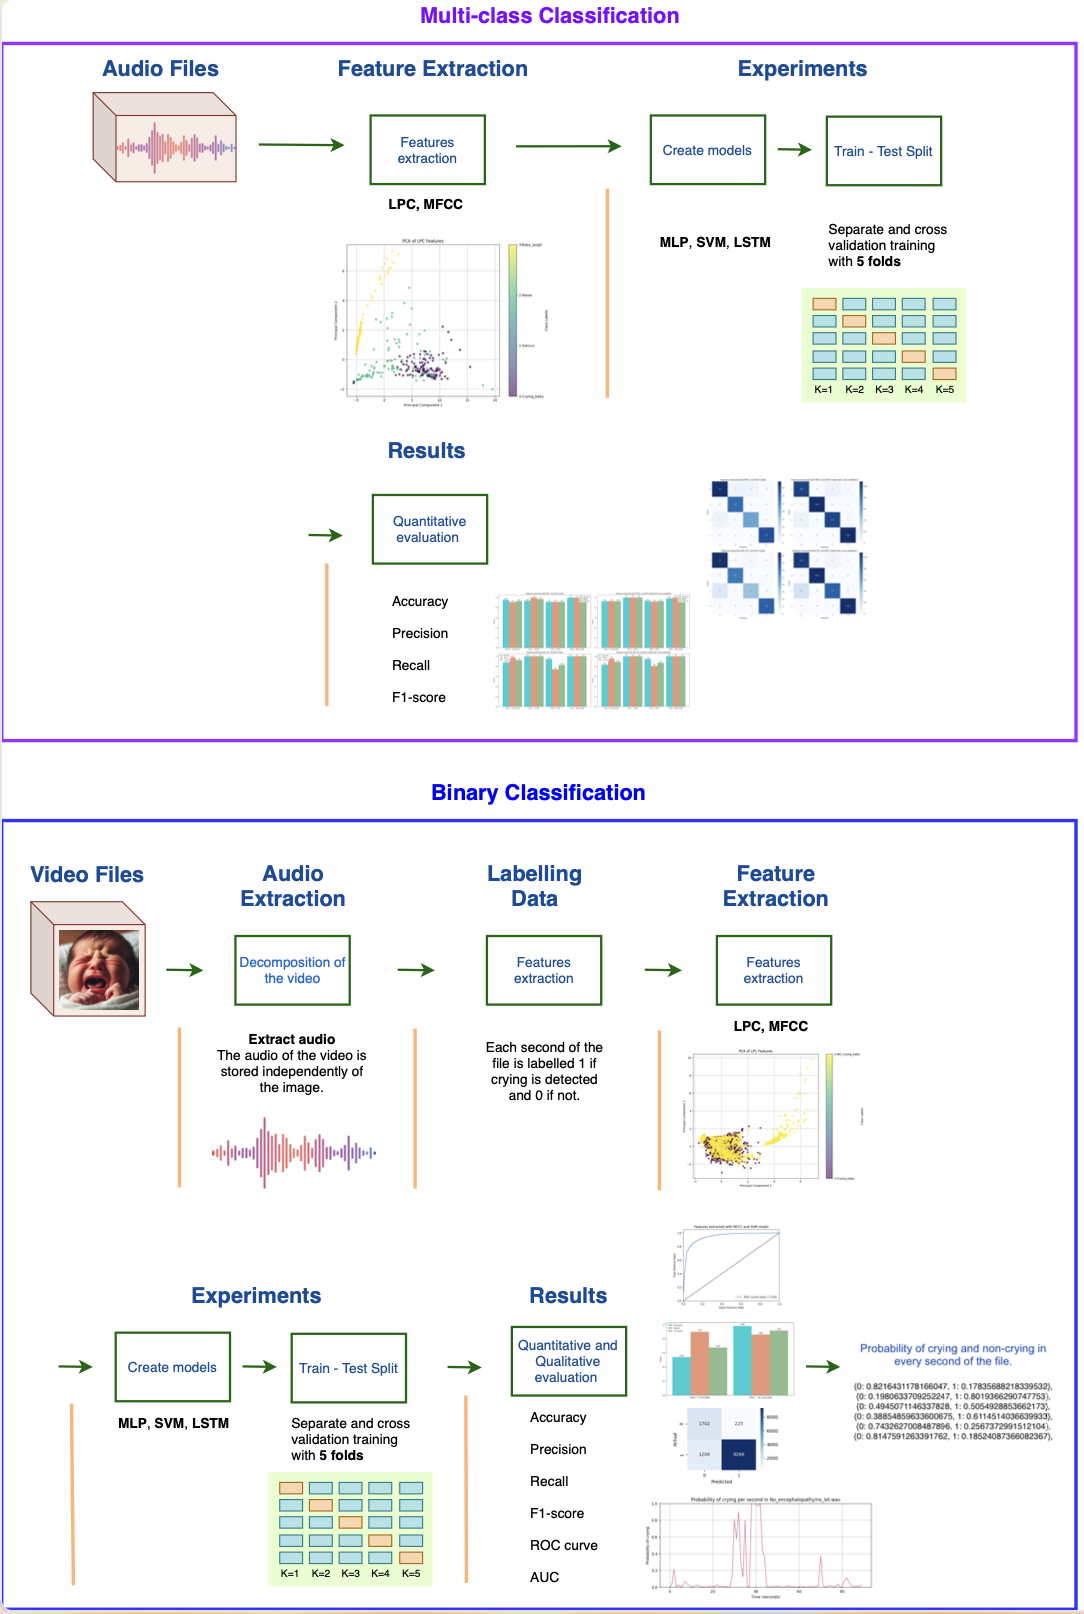
\includegraphics[width=0.9\textwidth]{figures/Project-Diagram.png}
\caption{General diagram of the project}
\label{fig:Project-Diagram}
\end{figure}

Finally, to validate the results obtained, \textbf{two validation strategies} were followed. The first was to evaluate the results using performance metrics. It should be noted that since these are binary classifications, the Receiver Operating Characteristic (\textbf{ROC}) curve, and the Area Under the Curve (\textbf{AUC}) have been calculated in addition to the common metrics, such as \textbf{accuracy}, \textbf{recall}, \textbf{precision}, and \textbf{f1-score}. The second strategy was to evaluate the models using the remaining five audios that were not previously used. Thereafter, a graph of the probability that the baby is crying in each second of the audio was developed.


\newpage
\section{Datasets}
This project worked with two datasets, first, a public one for initial testing, and the second, and most \textit{important}, a dataset provided by the University Hospital of Burgos. 

\begin{tcolorbox}
The public dataset was only used to assess the functionality and / or viability of the models in classifying infant crying. The dataset provided by HUBU is fundamental as it contains raw data with which the models will be trained to accurately, and precisely identify newborns’ cries.
\end{tcolorbox}

The first dataset comes from the public repository \myurl{https://github.com/giulbia/baby_cry_detection.git}{Baby Cry Detection} and its structure corresponds to the one shown in the image \ref{fig:public-dataset}. This dataset has the following four directories, each containing one hundred and eight (108) files with extensions (.ogg, and .wav): 
\begin{itemize}
    \item \textbf{Noise}, this directory can be considered the most diverse, and it contains files of different noises that any person can experience on a daily basis, for example, an animal bark, vehicle noises from the road, sounds such as birds singing, and those generated by church gongs, etc. 
    \item \textbf{Silence}, this directory contains audios that have no significant variation in amplitude over time. They are flat audios (such as white noise) and do not contain absolute silence but contain a series of sounds or noises that are not characterised by anything in particular.
    \item \textbf{Baby\_laugh}, this directory has files that contain the laughter of different babies. Unlike crying, the laughter tends to be softer, and more musical without a great intensity or presence of peaks in volume.
    \item \textbf{Crying\_baby}, this directory has files containing the cries of different babies. Unlike the previous directory, a baby's cry has a higher pitch, and is more variable in frequency compared to a laugh, and this distinction makes the machine learning models effectively differentiate them.
\end{itemize}

\begin{figure}[h]
\centering
    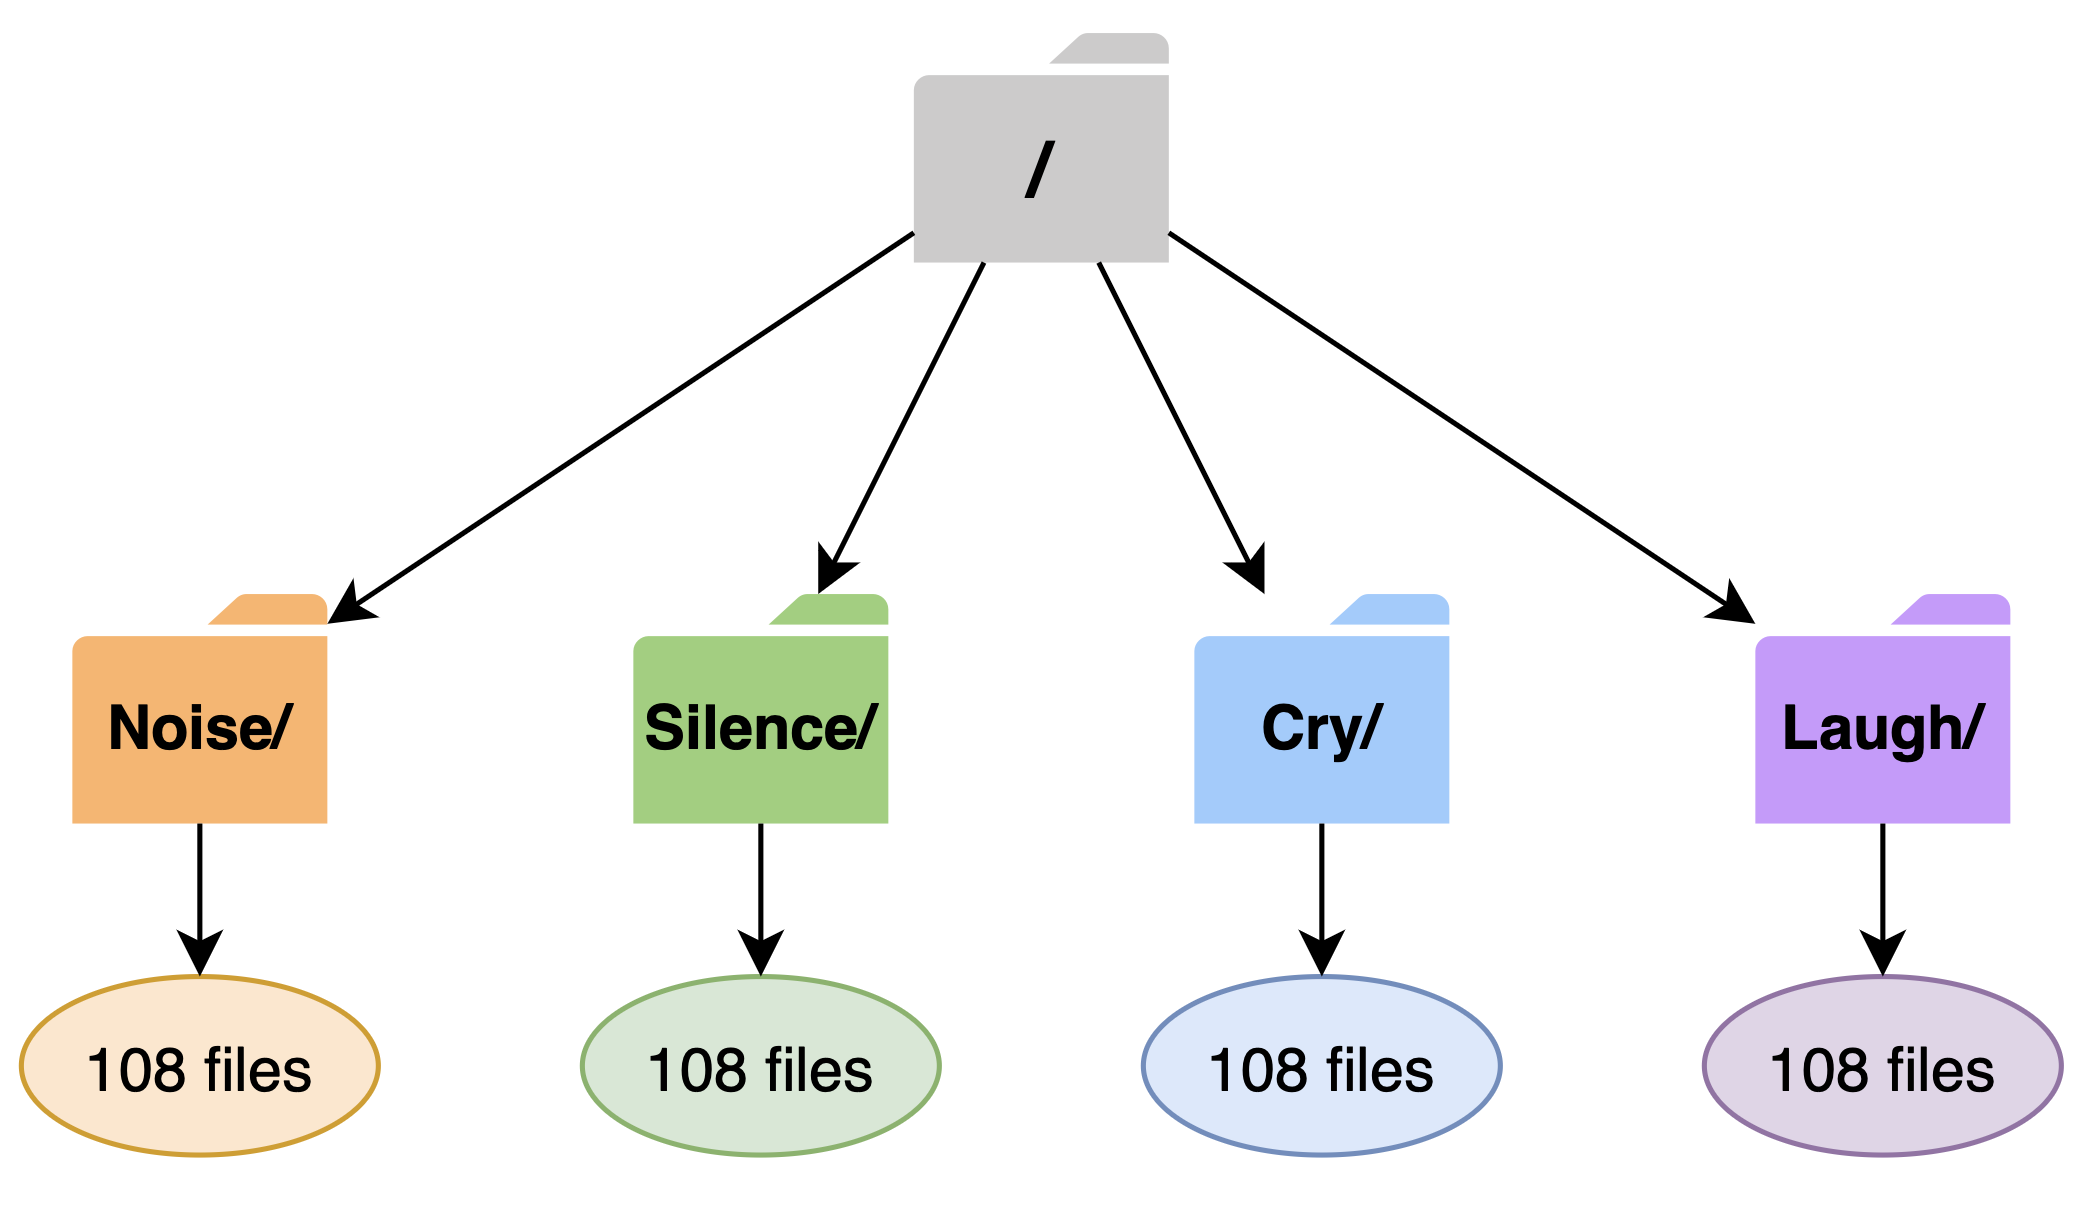
\includegraphics[width=0.5\textwidth]{figures/DirectoryPublicData.png}
\caption{Directory structure of the public dataset}
\label{fig:public-dataset}
\end{figure}

As can be seen in the previous files, there is a notable mixture of sounds, which can be essential for a precise identification of crying. However, the models will inevitably have some inefficacies in identifying cries since the audios from the public dataset are so ideal, yet the audios they are eventually trained with are more typical or representative of the environment (i.e. health setting). 

The second dataset contains a total of \textbf{sixty-three (63) files} provided by the maternity ward of the \textbf{University Hospital of Burgos}. These are video files of newborns babies’ responses, and reactions to differences stimulus presented by health workers to detect HIE. All these babies were born in 2023, and were less than twenty-four (24) hours old, at the time the videos were made. Some of the babies were premature, and had underlying health conditions and / or complications during birth. For this reason, the cries in this dataset are diverse, and this is key in training the models. 

The videos vary in length, ranging from videos as short as thirty seconds and up to sixteen-minutes. Them were captured using two different smartphones, each one with different image properties. Firstly, one set of videos (stored as .mov files) was obtained at a frame rate of 29.89 frames per second (FPS), with each frame having a resolution of 1920 x 1080 pixels. Secondly, another set of videos (stored as .mp4 files) was recorded using a different smartphone at a frame rate of 30 FPS and a resolution of 848 x 480 pixels. However, the audio characteristics remained consistent in both sets of videos. Both sets were recorded using two audio channels and a sampling rate of 44.1 kHz.

The videos from the previous paragraph demonstrate how the HUBU medical staff perform a thorough examination of the newborn or a portion of it. The complete examination consists of numerous stimuli to which the baby must make a response, such as checking whether it’s gaze follows a presented object or whether it generates the involuntary movements that are expected in response to a given stimulus. However, in this project, the videos in which a small pinch is performed on the baby to elicit a cry were the main focus. Also, the cry’s characteristics such as duration, pitch, continuity or progressiveness, and whether the crying stopped abruptly were also key considerations.

\begin{tcolorbox}
It is important to note that although the videos contain audio with some details, and indications from the doctor about the newborns’ conditions, the audio has only been used to analyse crying in this project. In addition, it is worth mentioning that in the absence of prior information related to the videos, it was so crucial to carry out labelling as part of the pre-processing of the study data.
\end{tcolorbox}

The directory system that was created with the videos is shown in the image \ref{fig:HUBU-dataset} and has the following five directories:
\begin{itemize}
    \item \textbf{Unclassified}, this directory contains a total of 58 videos with different lengths and video formats. In the videos, medical personnel can be observed exposing the neonates to different stimuli.  Sometimes the video contains a single stimulus, thus the shorter files, and on other occasions several stimuli which generates longer files.
    \item \textbf{Severe\_encephalopathy}, this directory contains a single video file of a newborn with severe signs of encephalopathy, which means that this baby does not cry at all when exposed to various stimuli. The video lasted 16 minutes and 54 seconds. 
    \item \textbf{Moderate\_encephalopathy}, this directory contains a single file with a duration of 90.7 seconds. In it, the same stimulus with varying intensity, is repeated up to three times on the neonate, to test its response to the pain.
    \item \textbf{Mild\_encephalopathy}, this directory contains a single video file of a newborn baby exposed to different stimuli. Due to its long duration, audio was extracted and divided into a series of clips that represent each of the stimulations given to the newborn. This was to evaluate more precisely whether the models correctly classified the moments in which the newborn cried.
    \item \textbf{No\_encephalopathy}, this directory contains two video files of 89.4 and 55.08 seconds. These files contain the stimulations performed on two different babies. Due to their healthy state, their response to the presented stimuli is that of an intense cry.
\end{itemize}

As can be seen in the file system above, most of the videos are unclassified in terms of the degree of the babys’ encephalopathy. This was not an issue encountered in this project, since the general objective was to be able to detect whether the baby had HIE or not by means of data analysis. Nevertheless, this isn’t the main objective of this project which is, to precisely detect whether a baby cries or not at any given time, when exposed to stimuli in a health setting. Additionally, it should be noted that the absence of crying is not a conclusive indicator of a positive HIE diagnosis. An example is some of the babies tested (exposed to stimuli) for HIE in the HUBU videos who had been intubated, could not cry, and this did not necessary mean they had HIE. 

\begin{tcolorbox}
All videos used in this study were acquired with the written consent of the newborns’ parents, who voluntarily provided their babies’ data, to contribute to the advancement of the study of HIE. However, due to privacy and data protection laws, this project will not include the original videos, audios, or images that would allow identification of the babies, nor will names or any other data that could facilitate identification of the study participants or their family members be released.
\end{tcolorbox}

\begin{figure}[h]
\centering
    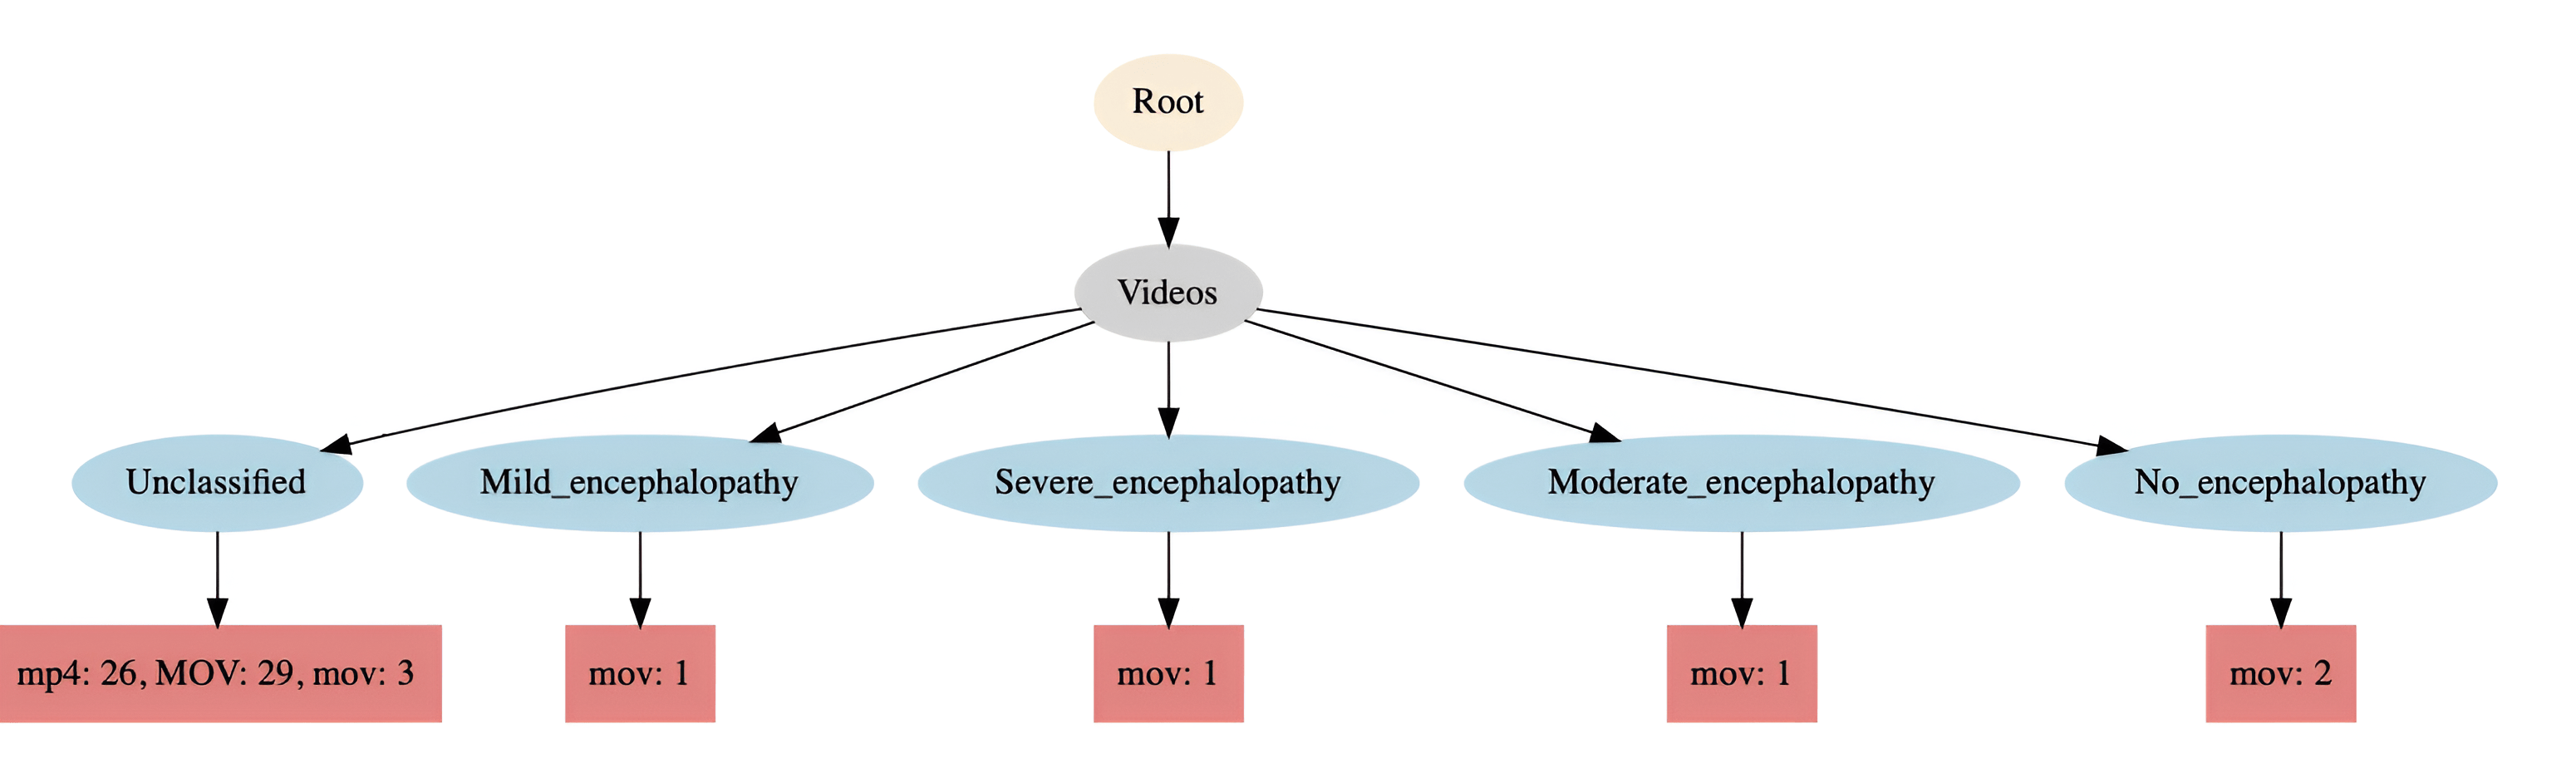
\includegraphics[width=1\textwidth]{figures/directory-HUBU.png}
\caption{Directory structure of the HUBU dataset}
\label{fig:HUBU-dataset}
\end{figure}

\newpage
\section{Data Preparation}
The first step to work with audio in this project was to separate the video from the audio. This process is available on GitHub in the notebook \myurl{https://github.com/lnc1002/TFM-Newborn_Cries_Classification/blob/06473b645fd3b11fd7c81186fe494e7f3e4469ed/src/1)\%20First_steps/1_Notebook-1_Audio_Extraction.ipynb}{/src/1)First\_steps/1\_Notebook-1\_Audio\_Extraction.ipynb} where the audio extraction from the video can be appreciated using the \textbf{PyDub} Python library. Next, a directory system has been created, as shown in the image \ref{fig:directory-audios}, to store the audio files. In this way, a quick association between the extracted audio, and the original videos is achieved. 

All the extracted audio files have the extension \textbf{.wav} and the original name of the different files has been preserved. This has been done with the aim of subsequently creating a dataset that includes the different responses captured in relation to stimuli performed, i.e. for each file a list of the time frame in which the eyes and mouth remain open, the frown, and the baby's cry.

\begin{figure}[h]
\centering
    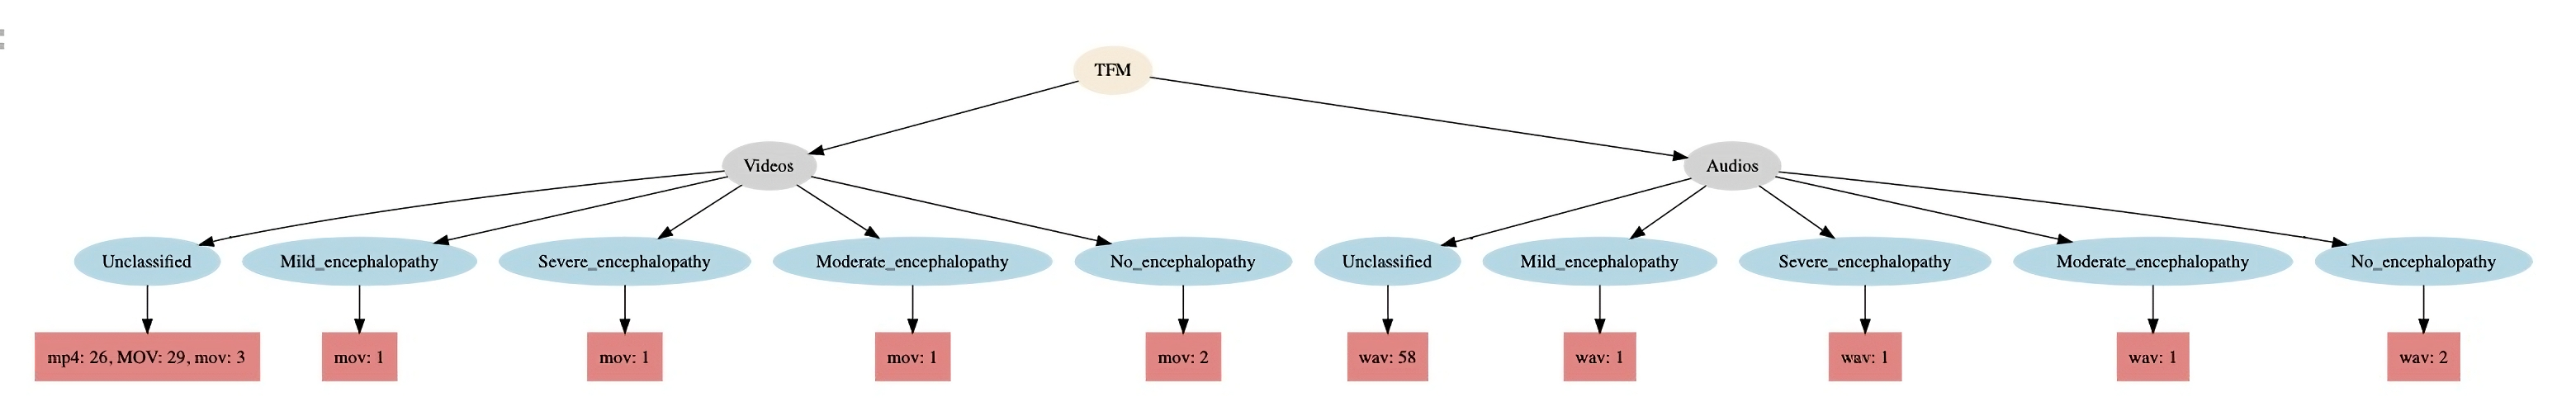
\includegraphics[width=1\textwidth]{figures/directory-with-audio.png}
\caption{Directory structure together with the extraction of audios from the HUBU dataset}
\label{fig:directory-audios}
\end{figure}

The way in which the data has been labelled also needs to be emphasised. For this purpose, a code has been developed that automates the process based on the duration of the audio in seconds. This code generates an array containing \textbf{binary values}, where a value of \textbf{0 indicates that the baby is crying} and a value of \textbf{1 indicates that the baby is not crying}. This vector is created in such a way that it has as many values as there are seconds in the audio, providing an accurate and granular representation of the baby's behaviour over time.

This process is simple to perform, in fact, it can be done manually by directly assigning 0s and 1s according to the baby's crying. In any case, the code has been very useful due to the fact that sometimes there are very long audios in which entering values by hand is tedious, especially when the time intervals in which the crying is appreciated are minimal. Despite its great usefulness, due to its simplicity and lack of direct relevance to this project, it has been decided not to show this code and to make only the generated files available to the user. 

In the notebook \myurl{https://github.com/lnc1002/TFM-Newborn_Cries_Classification/blob/4d0c85c8b15c2c117ca147f7c9625d47ff986ad8/src/1)\%20First_steps/2_Notebook-2_Basic_Operations.ipynb}{/src/1)First\_steps/2\_Notebook-2\_Audio\_Basic\_Operations.ipynb} the tags that have been created are exposed. As mentioned above, the data is structured in directories, with the \textit{Unclassified} directory having the most data available. For this reason the labels are stored in several text files: \textit{Unclassified\_data.csv} (contains the labels for the audio files in the \textit{Unclassified} directory), \textit{Test\_data.csv} (contains the labels for the audio files in the other directories, those that classify the baby's cry according to the type of HIE) \textit{Mild\_encephalopathy\_clips.csv} (contains the labels for the audio clips in the \textit{Mild\_Encephalopathy} directory).

\vspace{\baselineskip}

\begin{tcolorbox}
The audio file available in the \textit{Mild\_Encephalopathy} directory is composed of several time instants of baby crying, but the duration of this file is rather long. For this reason, so that later in the final qualitative analysis it is possible to clearly observe the instants of time in which the baby is crying, it has been decided to create \textbf{nine clips} with the different stimulations that are performed on the baby. These clips consist of dividing the audio according to the instants of time in which the baby begins and ends with a stimulation. 
\end{tcolorbox}

\newpage
It is very important to note that this type of labelling is very simple and the results may appear to be inaccurate in some cases. Unlike the models that have been trained and evaluated in this project, this labelling does not give a probability that the baby is crying but a single value, regardless of the amplitude of the sound, e.g. at the beginning or at the end of crying.


\section{Feature Extraction}
After reviewing the existing literature on which techniques should be used to classify infant crying, this section will present the techniques applied for the extraction of characteristics. The first technique, \textbf{MFCC}, has been referenced in many articles, so it was essential to implement it. The second technique, \textbf{LPC}, has been referenced in some articles and in this study it has been tested in order to create a comparison with the previous technique and to check how much better results it can offer. 

\begin{tcolorbox}
The public dataset has a total of four classes (Crying\_baby, Silence, Noise, Baby\_laugh) and the dataset provided by the HUBU has two classes (Baby\_cry, Baby\_not\_cry).
\end{tcolorbox}

\subsection{Mel Frequency Cepstral Coefficients (MFCC)}
Feature extraction using Mel Frequency cepstral coefficients (\textbf{MFCC}) is a complex process by which an audio signal is transformed from its original time domain to a representation that mimics the human perception of sound. The resulting coefficients represent the shape of the spectral envelope of the sound in the domain of the logarithm of the Mel frequencies \cite{Abdul2022}.

\begin{tcolorbox}
These are a good choice for audio analysis and sound classification because they provide a representation that mimics the way humans perceive sound.
\end{tcolorbox}
\vspace{\baselineskip}
This feature extraction process can be broken down into several key steps as shown in the image \ref{fig:MFCC-diagram}.

\begin{figure}[h]
\centering
    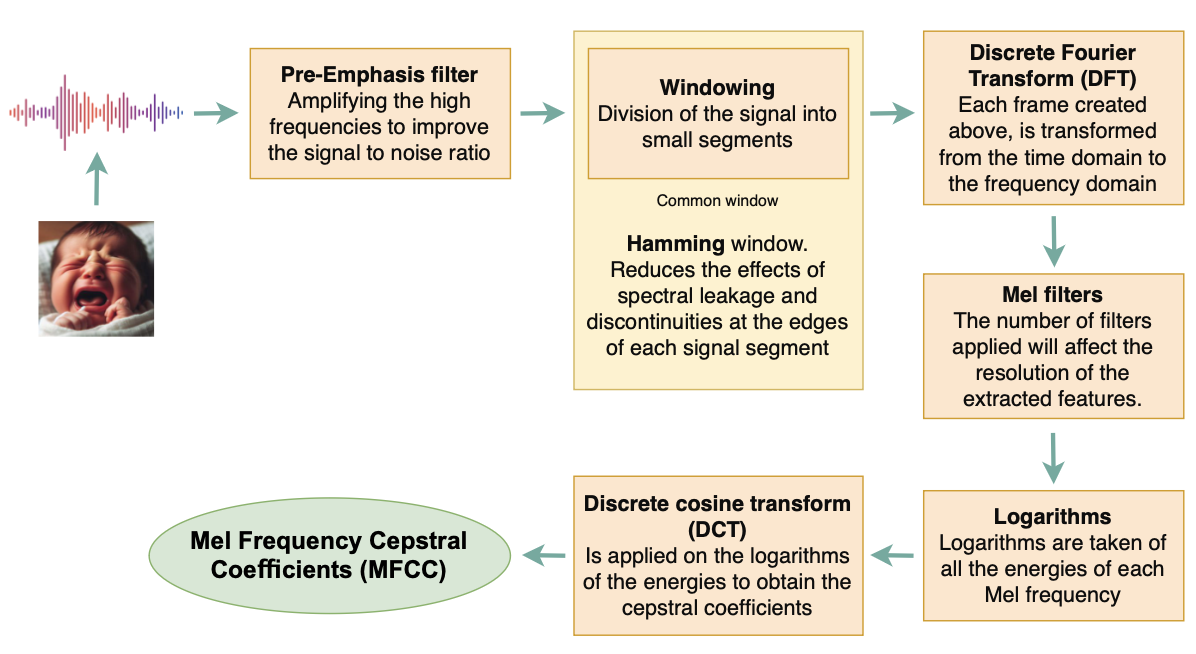
\includegraphics[width=1\textwidth]{figures/MFCC-diagram.png}
\caption{Diagram of the MFCC Feature Extraction Process}
\label{fig:MFCC-diagram}
\end{figure}
\vspace{\baselineskip}
\begin{tcolorbox}
These values that have been obtained are the MFCC coefficients that were sought to capture the most important characteristics of the audio signals. The objective of these coefficients is to identify the relevant content by ignoring information of little value, such as background noise, which does not contribute anything to the recognition process, on the contrary, it impoverishes it.
\end{tcolorbox}

\newpage

{\fontsize{16pt}{16pt}\textcolor{gray}{\textbf{MFCC implementation}}}

The Python library \textbf{librosa} has been used to implement a feature extraction based on MFCC. This library is widely used in audio processing tasks due to its efficiency and ease of use. Its implementation is available in the notebook \myurl{https://github.com/lnc1002/TFM-Newborn_Cries_Classification/blob/4d0c85c8b15c2c117ca147f7c9625d47ff986ad8/src/3)\%20Final_steps/7_Notebook-7_Extract_Binary_Features.ipynb}{3)Final\_steps/7\_Notebook-7\_Extract\_Binary\_Features.ipynb}.

The first step has been to load the audio files with a specific sample rate, in this case a \textbf{sample rate of 44100Hz} has been set, which means that the audio is re-sampled at 44100 Hz during the loading. This sampling rate is that of each file in the dataset provided by the HUBU. However, for the sake of clarity, it has been decided to specify it because the librosa library detects whether or not the sampling rate of the file needs to change in order to start re-sampling, so unnecessary processing is not generated. 

The second step has been to \textbf{divide the audio into one-second segments}, where each of these segments have a length equal to the previously defined sampling rate. Each of these segments is checked for sufficient length, at least 2048 samples. This step has been carried out in order to apply the \textbf{Hamming} window correctly, which the \textbf{librosa} library uses internally, and subsequently the Discrete Fourier Transform (DFT).  After this check, the process is continued by extracting, in this case, \textbf{thirteen MFCC coefficients} for each segment. The choice of this number of coefficients is given by the objective pursued by the project. This value provides a balance between information and computational efficiency, being sufficient for speech processing tasks. 

Finally, the result obtained is an average of the coefficients over time for each segment, so that each second of audio becomes an independent instance with fixed-length characteristics. \textbf{In this way, the models are subsequently provided with consistent data for training}. 

\subsection{Linear Predictive Coding (LPC)}
Linear Predictive Coding (\textbf{LPC}) feature extraction works in a very similar way to MFCC. Although both techniques divide the signal into frames and apply a window to reduce edge effects, they differ significantly in how they process those frames to extract features. LPC models the signal as a linear combination of its previous samples and uses autocorrelation to estimate the predictive filter coefficients \cite{Bradbury2000}.

\begin{tcolorbox}
This type of feature extraction attempts to model the human production of sound rather than transmitting an estimation of the sound wave. 
\end{tcolorbox}

This feature extraction process can be divided into several key steps, as shown in the image \ref{fig:LPC-diagram}.

\begin{figure}[h]
\centering
    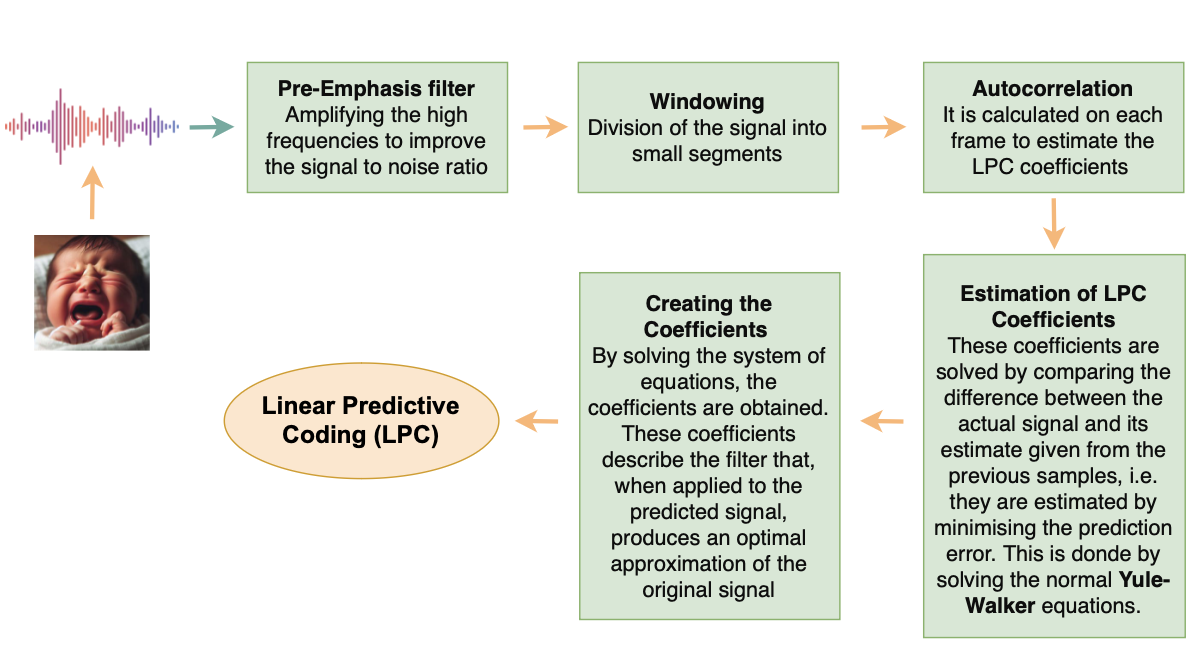
\includegraphics[width=1\textwidth]{figures/LPC-diagram.png}
\caption{Diagram of the LPC Feature Extraction Process}
\label{fig:LPC-diagram}
\end{figure}


{\fontsize{16pt}{16pt}\textcolor{gray}{\textbf{LPC implementation}}}

As in the previous case, the Python library \textbf{librosa} is still used for feature extraction, in this case based on LPC. The implementation is available in the notebook \myurl{https://github.com/lnc1002/TFM-Newborn_Cries_Classification/blob/4d0c85c8b15c2c117ca147f7c9625d47ff986ad8/src/3)\%20Final_steps/7_Notebook-7_Extract_Binary_Features.ipynb}{3)Final\_steps/7\_Notebook-7\_Extract\_Binary\_Features.ipynb}.

The first step has been to load the audio files with a \textbf{sampling rate} equal to \textbf{44100Hz}. Then, the \textbf{pre-emphasis} filter has been applied to improve the signal to noise ratio. This filter follows the formula where \textit{alpha} is greater than 0 and less than 1.0 \cite{GrabVoice2024}. Typical values for \textit{alpha} are between 0.95 and 0.97, on this occasion a value of \textbf{alpha=0.97} has been selected with the intention of amplifying the high frequencies to not introduce excessive distortion into the signal. 

Afterwards, the audio has been segmented into \textbf{one-second fragments} and a \textbf{Hamming window} was applied to each segment. After the windowing, the next step was to apply the autocorrelation technique. In this case, the most relevant part for the LPC coefficients has been selected, i.e. the part related to the centre of the forward autocorrelation has been extracted. This step has been intended to capture the temporal structure of the signal, making it possible to determine the current samples from the previous samples. Since the LPC coefficients model the signal according to the linear combination of past samples, this is a fundamental step. 

Finally, the Toeplitz equation is solved using the Levinson-Durbin algorithm to obtain the LPC coefficients. These coefficients are stored in a list of vectors in which the length of each vector is equal to the number of coefficients previously defined, in this case the \textbf{number of coefficients} has been defined equal to \textbf{10}.  


\section{Evaluated Features}

This section presents the main methods to achieve dimensionality reduction, and to visualise the features extracted from the different available data. As explained in the previous section, the number of classes differs between the different data available, that is the multi-class dataset, and the binary dataset. 

When feature extraction techniques are applied on the data, such as those used in this project, that is \textbf{MFCC}, and \textbf{LPC}, each audio sample is transformed into a set of features such as cries, laughs, and silences that detail essential information about the sound. The number of features vary, and depend on the extraction parameters such as the number of coefficients that are defined prior to extraction. 

In the case of the \textbf{MFCC} features extracted from the HUBU data, a total of 1239 features, and labels have been obtained per audio sample, which means that each sample in the dataset has been represented as a point in a space of 1239 dimensions. Each of these dimensions contains a specific aspect of the audio signal, such as the frequency of the formats, the energy in different frequency bands, etc. Having numerous features has a positive effect on the result, as it allows a more detailed representation of the sound, although, of course at the cost of a higher complexity of the results. 

For this reason, it is essential to apply dimensionality reduction techniques to be able to observe the results summarised in the image \ref{fig:pca-tsne-umap}. In this case, three techniques have been utilized i.e., Principal Component Analysis (\textbf{PCA}), t-Distributed Stochastic Neighbor Embedding (\textbf{t-SNE}), and Uniform Manifold Approximation and Projection (\textbf{UMAP}). All of them are available in the notebooks \myurl{https://github.com/lnc1002/TFM-Newborn_Cries_Classification/blob/4d0c85c8b15c2c117ca147f7c9625d47ff986ad8/src/2)\%20Second_steps/3_Notebook-3_Extract_Features.ipynb}{2)Second\_steps/3\_Notebook-3\_Extract\_Features.ipynb}, and \myurl{https://github.com/lnc1002/TFM-Newborn_Cries_Classification/blob/4d0c85c8b15c2c117ca147f7c9625d47ff986ad8/src/3)\%20Final_steps/7_Notebook-7_Extract_Binary_Features.ipynb}{3)Final\_steps/7\_Notebook-7\_Extract\_Binary\_Features.ipynb}, and are described in the next paragraphs.  


\textbf{Principal component analysis (PCA)} is a technique that consists of projecting observations from a \textit{p-dimensional} space where \textit{p} is the number of variables to a \textit{k-dimensional} space in which \textit{k} must be strictly less than p \cite{Paul2013}. This transformation models the set of possibly correlated variables into a set of uncorrelated variables called principal components \cite{Lipovetsky2009}. \textbf{The main objective of this technique is to keep as much information as possible while reducing the complexity of the data sets.} 

In this project, the \textbf{Scikit-learn} Python library has been used to provide an efficient implementation of PCA. Firstly, PCA was used to expose the data in two main components, thus creating a two-dimensional plane for visualisation. Then the data transformation is performed, and the scatter plot is drawn. This action has been performed with both MFCC, and LPC feature extraction methods. In the case of the features extracted with LPC some clustering of the data expressing the baby's non-crying can be observed, however, with MFCC the classes do not form clearly separated groups. 


\begin{tcolorbox}
These results are to be expected as for newborns’ cries, the cry is intermittent or discontinuous that is with varying amplitudes over time. This is on account of the intervals at which the baby inhales or exhales. Since amplitude at this point is low, the model might identify this timeframe as “non-crying”. This can result in inaccuracies as the model could interpret these instances as non-cries. This is why, although at first glance these results may not seem very encouraging, the truth is that they are the ‘expected’ ones.
\end{tcolorbox}

\newpage
Another technique \textbf{t-Distributed Stochastic Neighbor Embedding (t-SNE)} was used to compare the results. This technique consists of two main stages. The first stage focuses on the calculation of probabilities representing the similarities between pairs of points in a high-dimensional space. These probabilities indicate that closer pairs of points have a high probability of being selected together, as opposed to points that are far apart, which have a near-zero probability of being selected together \cite{arora2018analysis}. 


In the case of the features extracted with LPC some clustering of the data expressing the baby's non-crying can be observed, however, with MFCC the classes do not form clearly separated groups. 

The second stage focuses on mapping the obtained points to a lower-dimensional space, commonly two- or three-dimensional spaces. The aim is to make the similarities between the data in the lower dimension as representative as possible to those in the original space. This is achieved by minimising the Kullback-Leibler divergence between the probability distributions with respect to the locations of the points on the map. Once more, the classes are clustered, and do not end up forming clearly distinct groups.  For this reason, a final visualisation has been created to picture the results obtained in the previous feature distributions. 

\textbf{Uniform Manifold Approximation and Projection (UMAP)} is a Riemannian variant of t-SNE but, unlike t-SNE, it accomplishes a more effective balance by preserving local and global structures. This technique is mainly based on algebraic topology theory, which creates a projection of the high-dimensional data while preserving its topological structure. 

In this project we have used the \textbf{umap-learn} library that depends on Python's \textbf{Scikit-learn} to be able to observe the characteristics of the data by dimensionality reduction. The results obtained are similar to the ones obtained by the other previous techniques, and therefore, it is conclusive that these techniques are effective for a visual representation, but they are not enough to discriminate among classes effectively.

\begin{figure}[H]
\centering
    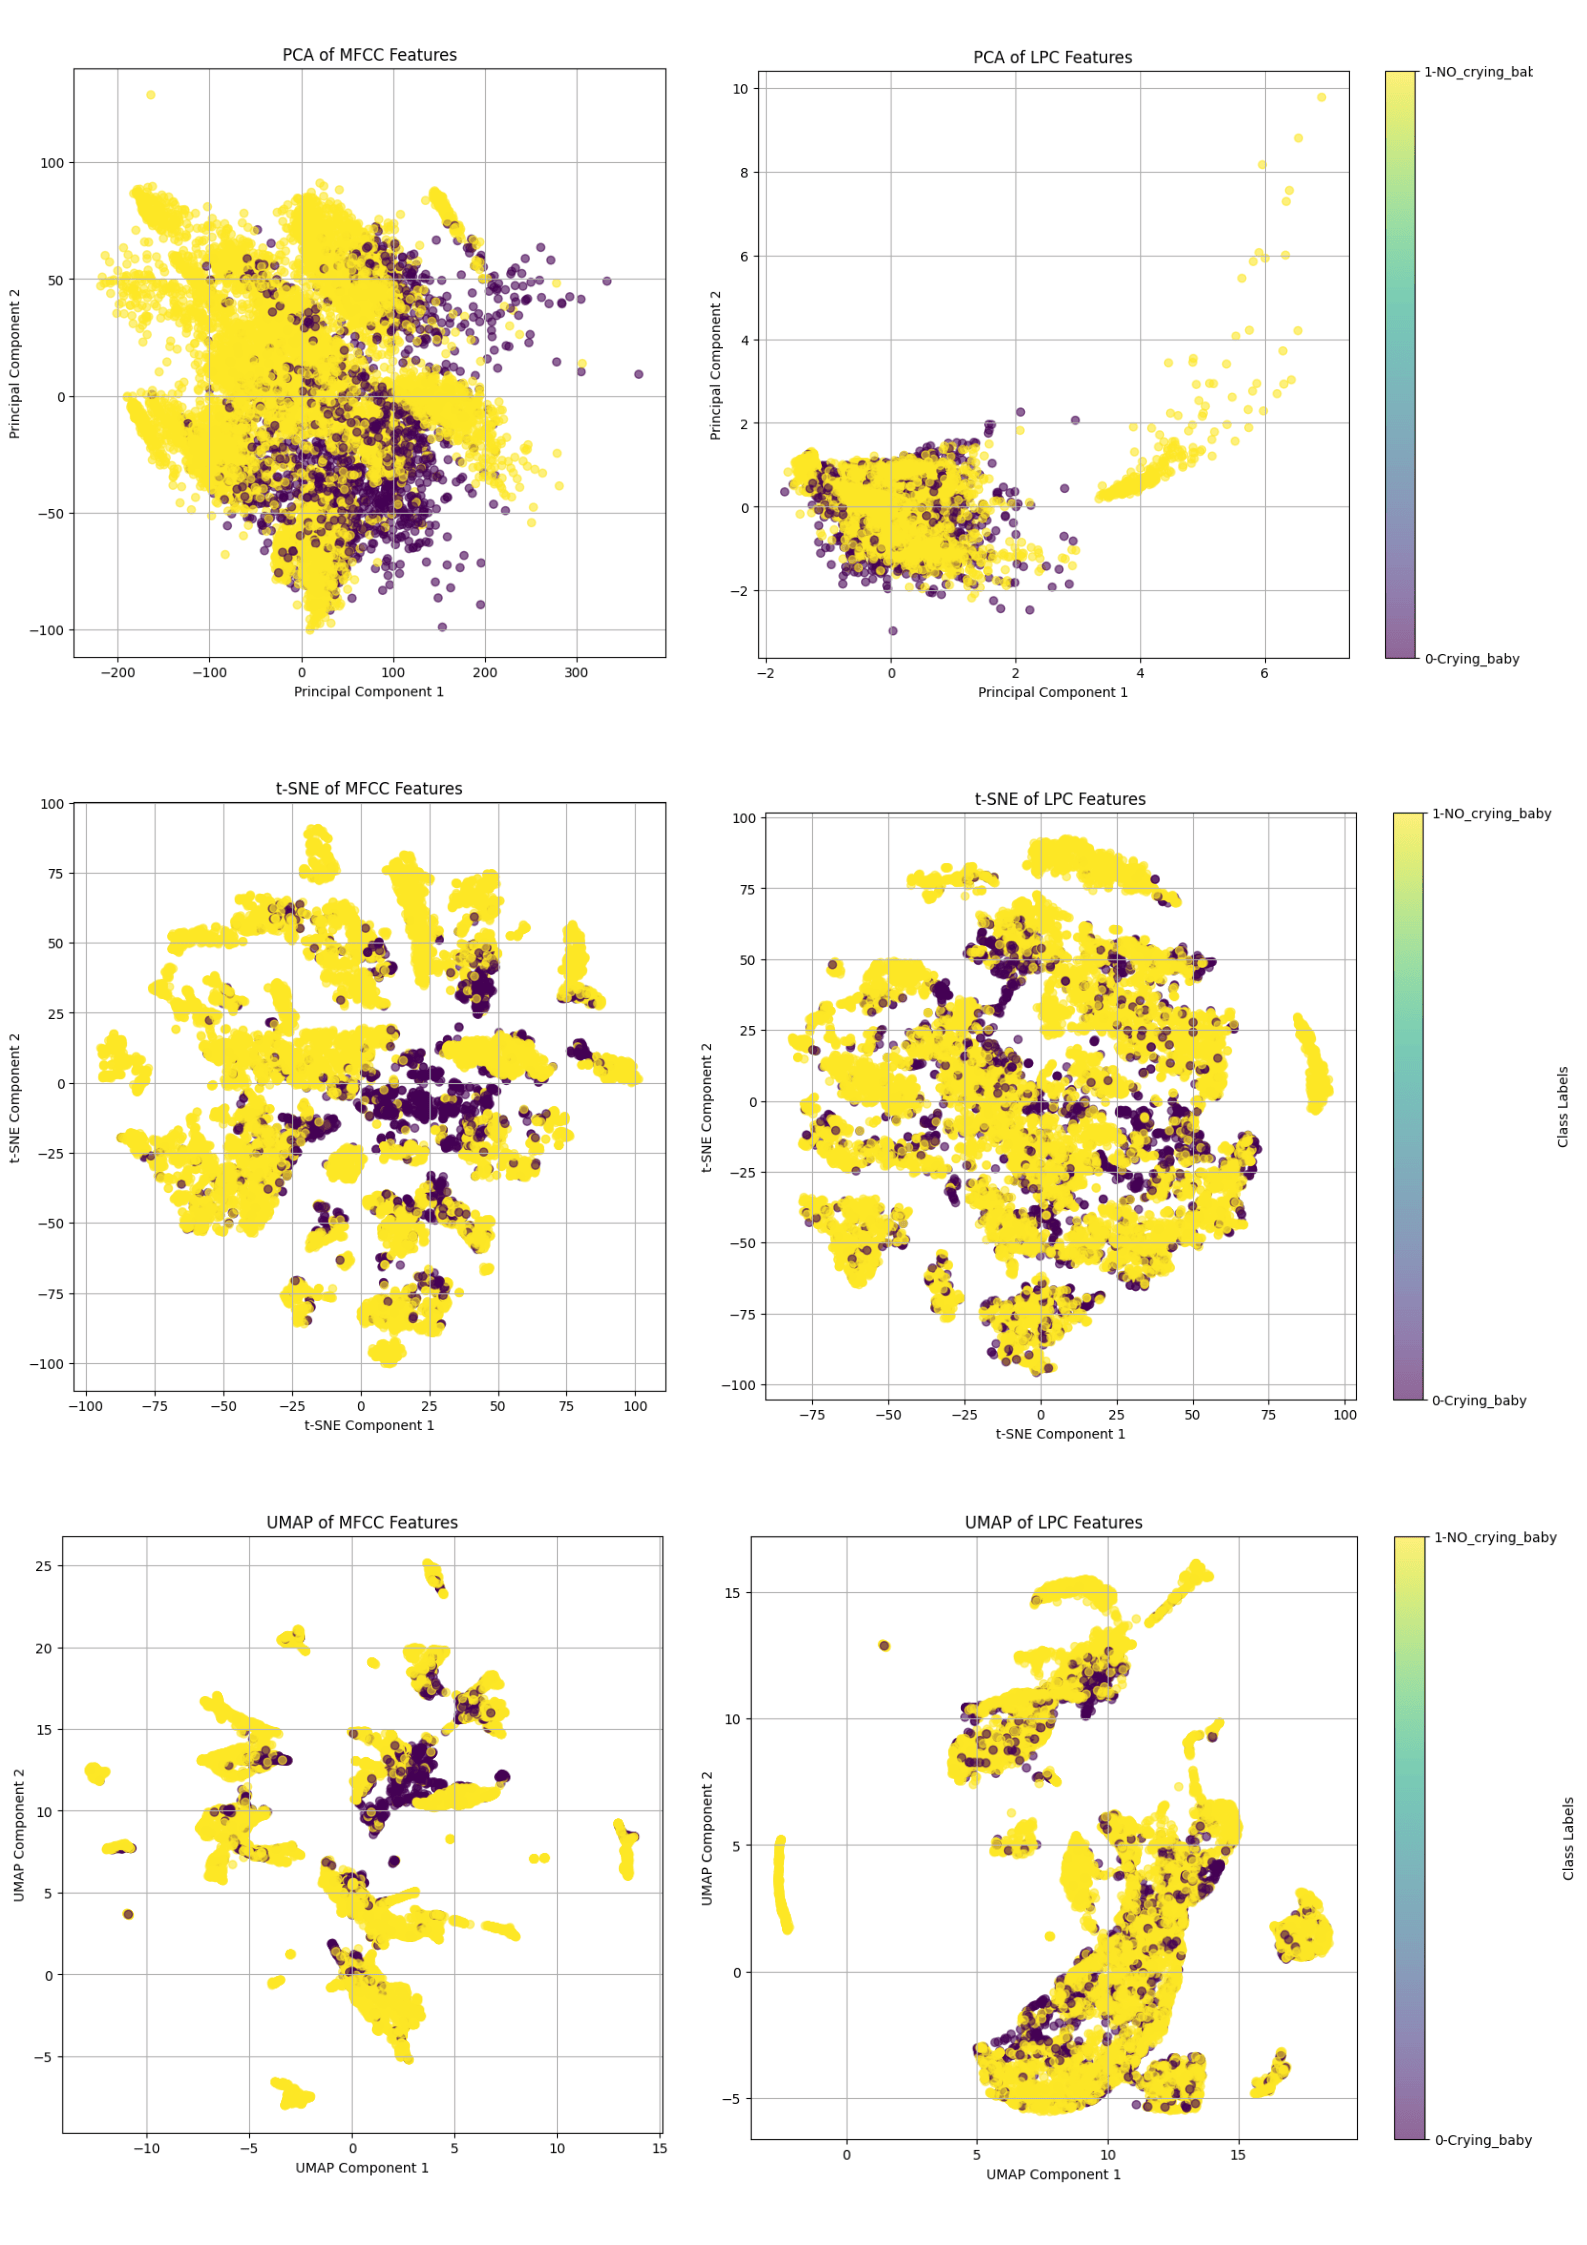
\includegraphics[width=0.9\textwidth]{figures/pca-tsne-umap.png}
\caption{Visualisation of the extracted features with different metrics.}
\label{fig:pca-tsne-umap}
\end{figure}

\section{Model Architectures and Implementation Details}

In the development of Machine Learning and Deep Learning models, it is as important to select the most appropriate models according to the type of classification being performed, as the way in which these models will be built and the techniques that will be applied to ensure their robustness and effectiveness. In this study, two fundamental aspects have been implemented: cross-validation and oversampling and undersampling techniques. 

Firstly, cross-validation is a resampling method based on the idea of dividing the dataset into k partitions, where in each of these partitions a test set is used only once, with the rest of the data being used for training. This process is repeated, rotating the allocation of the test data, so that at the end of the process all the data is used in both training and testing \cite{berrar2019cross}. 

\begin{tcolorbox}
The models have been trained with a total of 12399 MFCC and LPC features of which only 1927 (15.54\%) belong to the \textit{Baby\_cry} class and 10472 (84.46\%) belong to the \textit{Baby\_not\_cry} class.
\end{tcolorbox}

Most of the audios contain crying data only at the moment when the nociceptive stimulus\footnote{A nociceptive stimulus is a stimulus that activates pain receptors, usually due to tissue damage.} is performed on the baby, which causes most of the audio file to contain other non-crying sounds creating an unbalanced dataset in which the crying class is significantly under-represented. 


This problem is tackled in two different ways, the first is oversampling, extending the minority classes and the second is undersampling which reduces the number of samples in the majority class. In this project both techniques have been developed using \textbf{SMOTETomek} which is a hybrid technique combining \textbf{SMOTE} (Synthetic Minority Over-sampling Technique) for oversampling and \textbf{Tomek Links} for undersampling.


\subsection{Multilayer Perceptron (MLP)}
The Multilayer Perceptron (\textbf{MLP}) is a fundamental structure in the field of Artificial Neural Networks (ANN) due to the variety of solutions it presents for use in the field of machine learning. Its main characteristic is that it is capable of solving problems that are not linearly separable, which is also its main limitation \cite{Mercado2015}. This model consists of at least one input layer, one hidden layer and one output layer, as shown in the image \ref{fig:MLP-model}. In this same image it can also be seen how each layer is connected to the next by neurons.
\vspace{\baselineskip}

\begin{figure}[h]
\centering
    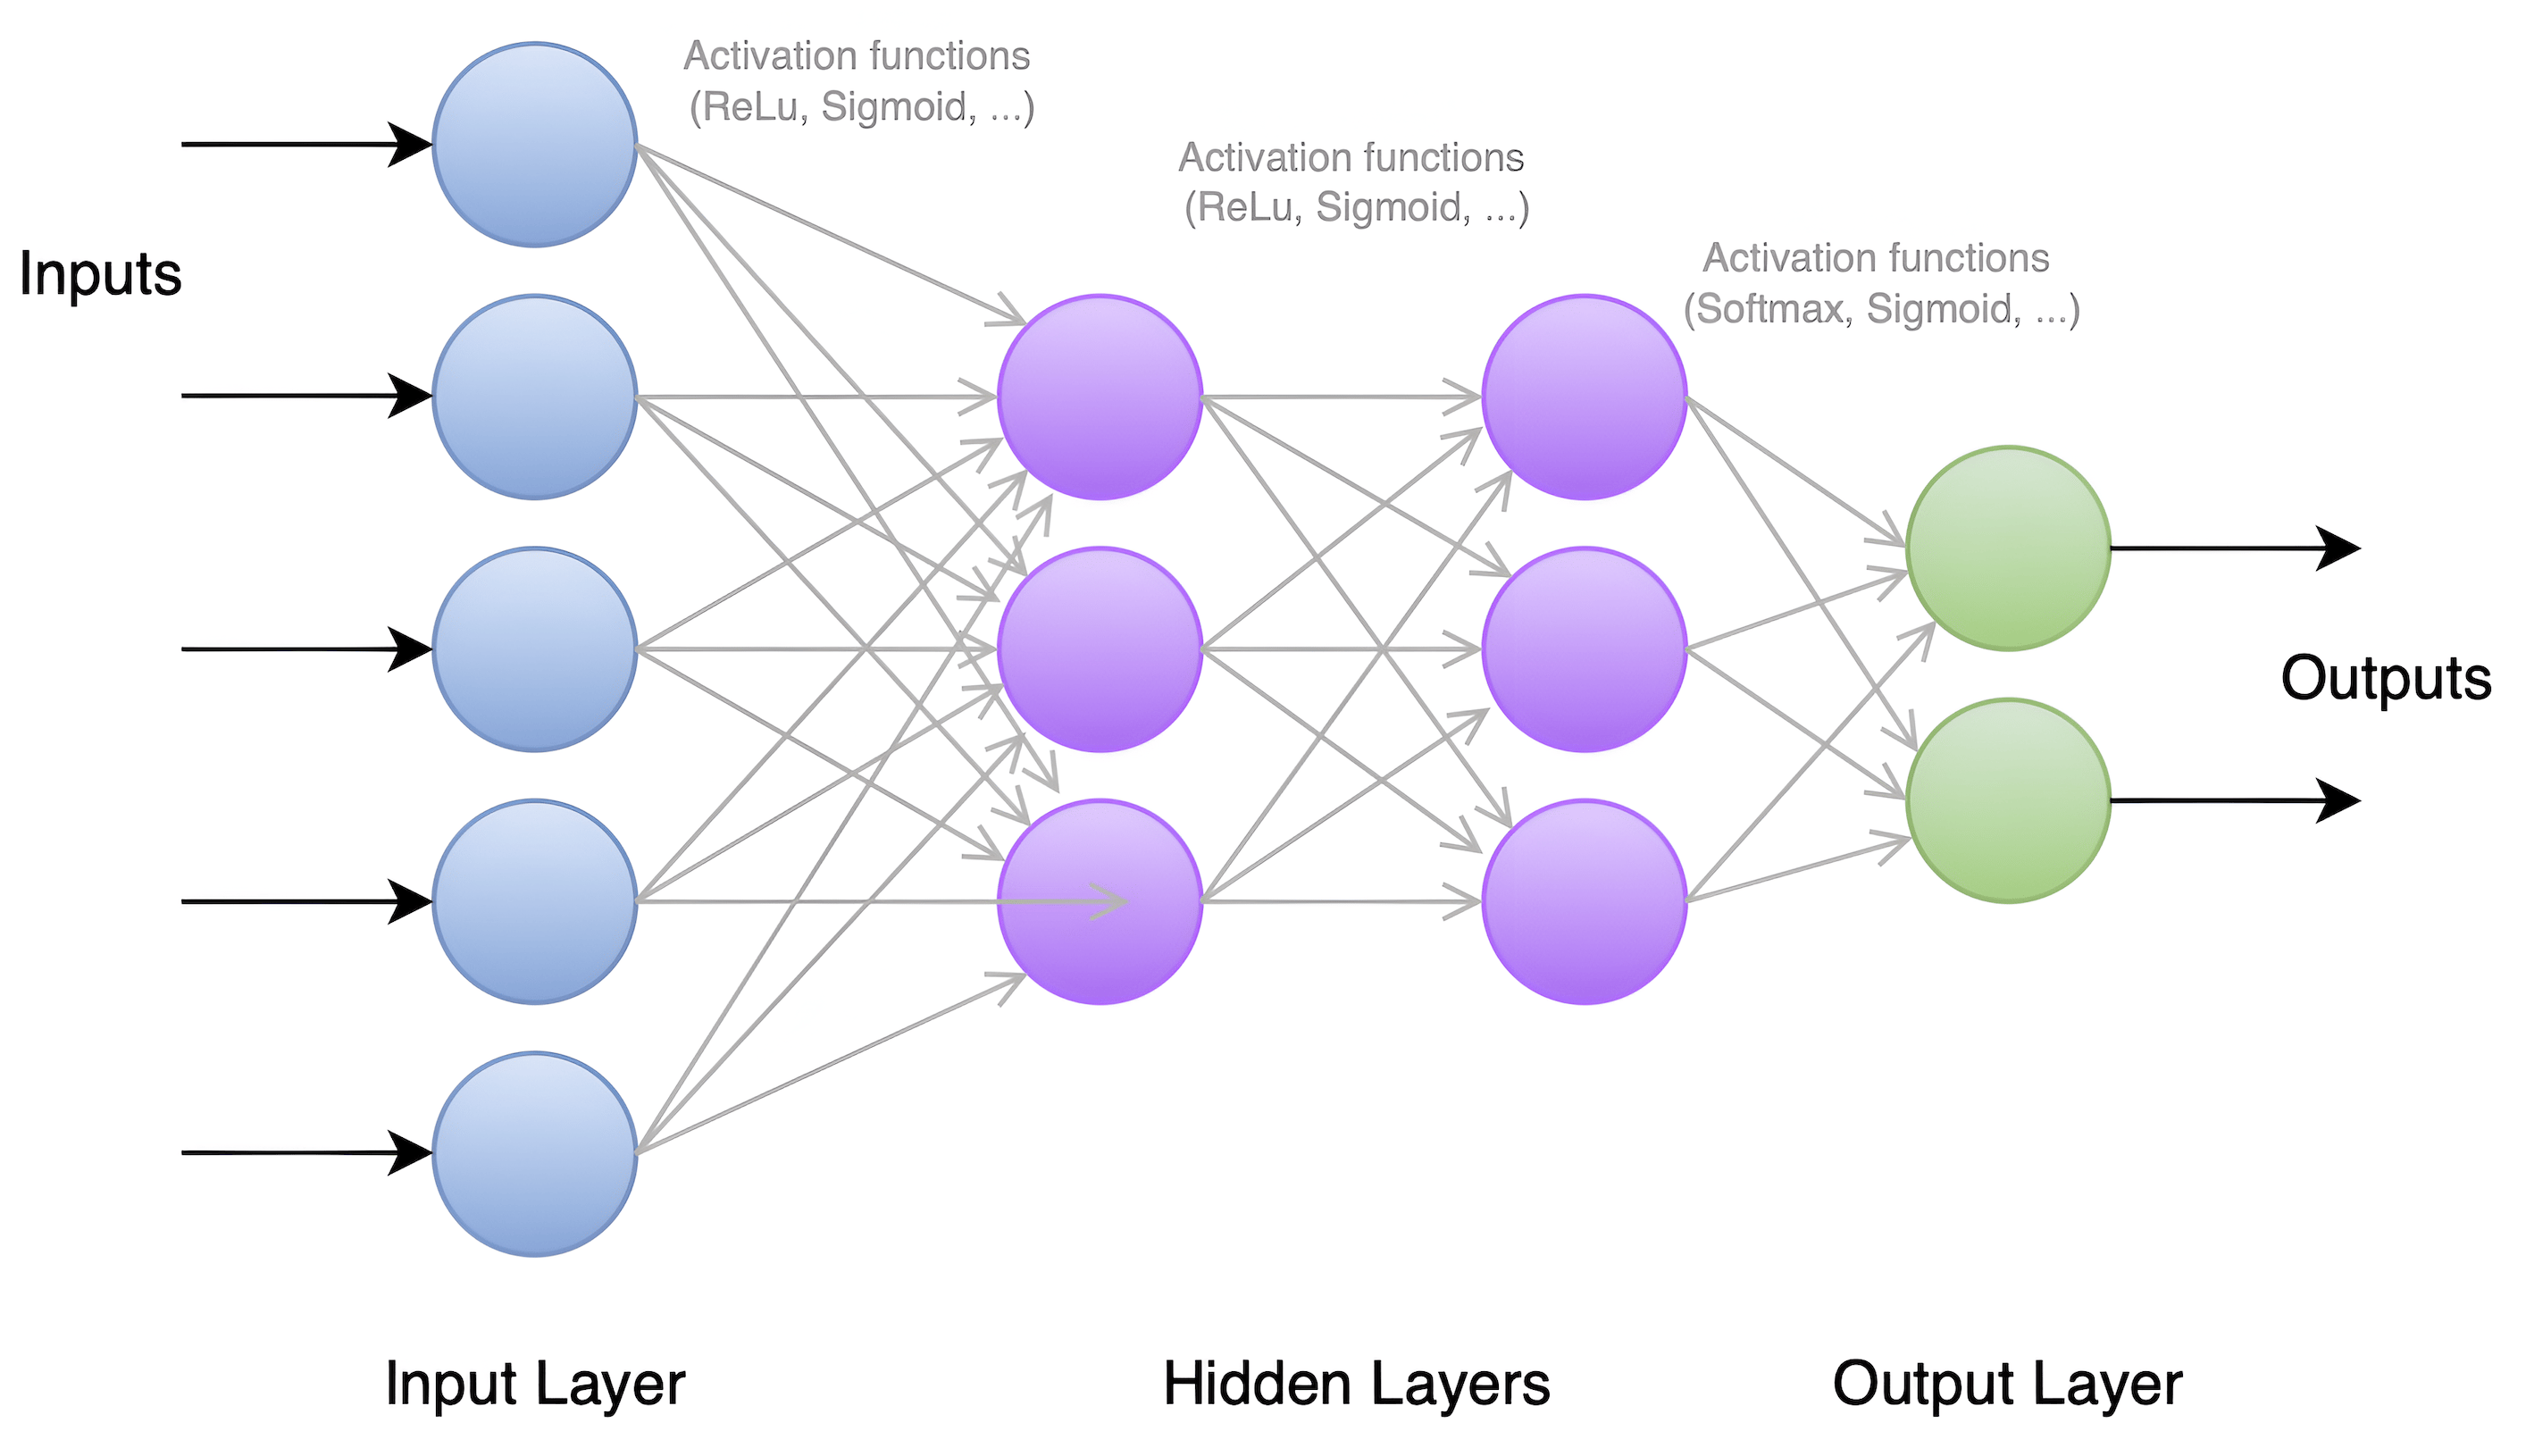
\includegraphics[width=1\textwidth]{figures/MLP-model.png}
\caption{Diagram of the MLP model}
\label{fig:MLP-model}
\end{figure}

\newpage

The \textbf{MLP} can have from one to several hidden layers but the neurons that compose this network have the particularity of only transmitting information forward through the network. For this reason, the operation of an MLP model can be broken down into the following steps \cite{popescu2019multilayer}: 
\begin{itemize}
    \item \textbf{Initialisation}, occurs at the input layer. This layer does not perform any computation on the input data, its mission is only to receive the information and distribute it to the subsequent layers. Each neuron in this layer will represent a characteristic of the input data set. 
    \item \textbf{Processing}, takes place in the hidden layers. These layers are considered the computational heart of the MLP model because this is where all non-linear processing operations perform. Neurons in this layer apply activation functions on the input data, some of the most common functions are \textbf{ReLu} (Rectified Linear Unit), which provides an output for all positive input values and \textbf{Sigmoid} which transforms all input values into the range [0-1], these sigmoid functions have the advantage of both nonlinearity and differentiation. 
    \item \textbf{Output}, which is produced in the output layer. This layer receives as inputs the outputs generated by the neurons of the last hidden layer and transforms this input into the final outputs of the model. As in the previous layer, this layer also has activation functions, and their use will depend on the distribution of data expected in the output. In this project, for the binary classification (0/1) that evaluates whether the newborn is crying or not, a \textbf{unipolar sigmoid} has been used. 
\end{itemize}

\vspace{\baselineskip}

\begin{tcolorbox}
The non-linearity of this model allows the network to be able to learn complex relationships and autonomously perform tasks that linear models are not capable of.
\end{tcolorbox}

\newpage
{\fontsize{16pt}{16pt}\textcolor{gray}{\textbf{MLP implementation}}}

The \textbf{MLP} model has been implemented in this project using the \textbf{Scikit-learn} library. This Machine Learning library is designed to be integrated well with other Python libraries, such as NumPy and SciPy, making it a competent and robust library for the purpose of this project. However, it should be noted that, although this library is not optimised to the same level of performance as the TensorFlow or PyTorch libraries, for researches such as the one which is being carried out in this project, it is a very competent alternative due to the moderate size of the data that has been collected to date. 
 
Creating a model with a good performance is crucial for any project, for this reason it must be taken into account how the different parameters of the neural network influence and how the different neurons behave during training. 

The artificial network that has been created consists on a \textbf{single hidden layer with 300 neurons}. The choice of a single hidden layer is driven by the limited amount of data available to date, the need to create a model with high computational efficiency and to meet the requirement that the risk of overfitting is minimised. On the other hand, using \textbf{MLPClassifier} the default activation function used for the hidden layers is the \textbf{ReLU} (Rectified Linear Unit) activation function, and it is the one that has been established due to the good performance it offers in deep learning problems. 

In addition, the parameters that affect the operation of all the neurons in the network must be robust to the values they contain, such as \textbf{adaptive weight adaptation}. This way the model will automatically adjust the learning rate if the training is not obtaining favourable results, i.e. if the model stops improving. Then, the \textbf{regulation parameter L2} affects all the neurons in the network except those in the input layer and penalises the larger weights in order to achieve a model that generalises better by promoting smaller weights. This parameter has been defined with a value of \textbf{0.01}, which allows for a balance between the model's ability to correctly fit the data while avoiding the risk of overfitting. 
 
Finally, the output layer is automatically selected according to the number of classes detected in the training of the model. If more than two classes are detected, the \textbf{softmax} activation function is automatically used. 


\subsection{Support Vector Machines (SVM)}

Support Vector Machines (\textbf{SVM}) belong to the category of linear classifiers because the method it implements is the creation of a hyperplane for the separation of the defined spaces. This separation can be done by means of two techniques, the first and simplest is the separation over the original space. In order to achieve this separation, the input examples have to be linearly separable. If these are not, it is necessary to create a transformed space, called feature space \cite{Mercado2015}. 

This supervised learning algorithm tries to find the best hyperplane in the input space among the existing classes, as can be seen in the image \ref{fig:SVM-model} which, being a two-dimensional representation, the hyperplane can be represented as a straight line. But this is not the only representation that can be made of this algorithm. If the representation is generated in three or more dimensions, the hyperplane becomes a plane that still aims to divide the classes with the maximum possible margin between them. 

The concept of this algorithm is actually a combination of computational theories that have existed for decades, such as hyperplane margins. These margins are defined as the smallest distance between the training points closest to the plane, known as support vectors, and the hyperplane. Achieving a robust margin boosts the model's ability to generalise unseen data, leading to greater confidence in the classification.  

The basic principle of SVM is that, although it was initially created as a linear classifier, it has been developed in such a way that it can also be used in non-linear problems. This modification is achieved by incorporating what are called kernel tricks. These kernels are defined as functions that allow the scalar product of two vectors in a transformed feature space to be calculated without having to compute the transformation. This makes it easier to operate with higher dimensional spaces where classes can be separated in a more efficient way without incurring computational costs. The most common kernels used in SVM are:
\begin{itemize}
    \item \textbf{Linear}, this type of kernel is the simplest as it makes no modifications to the input space and uses the scalar product as the similarity measure. 
    \item \textbf{Polynomial}, this type of kernel creates a polynomial feature space and is able to model non-linear and curved boundaries. A too low or too high degree can cause over-fitting or under-fitting.
    \item \textbf{Radial Basis Function (RBF)}, this kernel manages to project the data into an infinite dimensional space, being able to handle non-linear and multidimensional data although it can be sensitive to noise and outliers. 
    \item \textbf{Sigmoid}, this kernel applies a sigmoid function to the data mimicking the behaviour of a neural network with a sigmoid activation function.
\end{itemize}

\begin{figure}[h]
\centering
    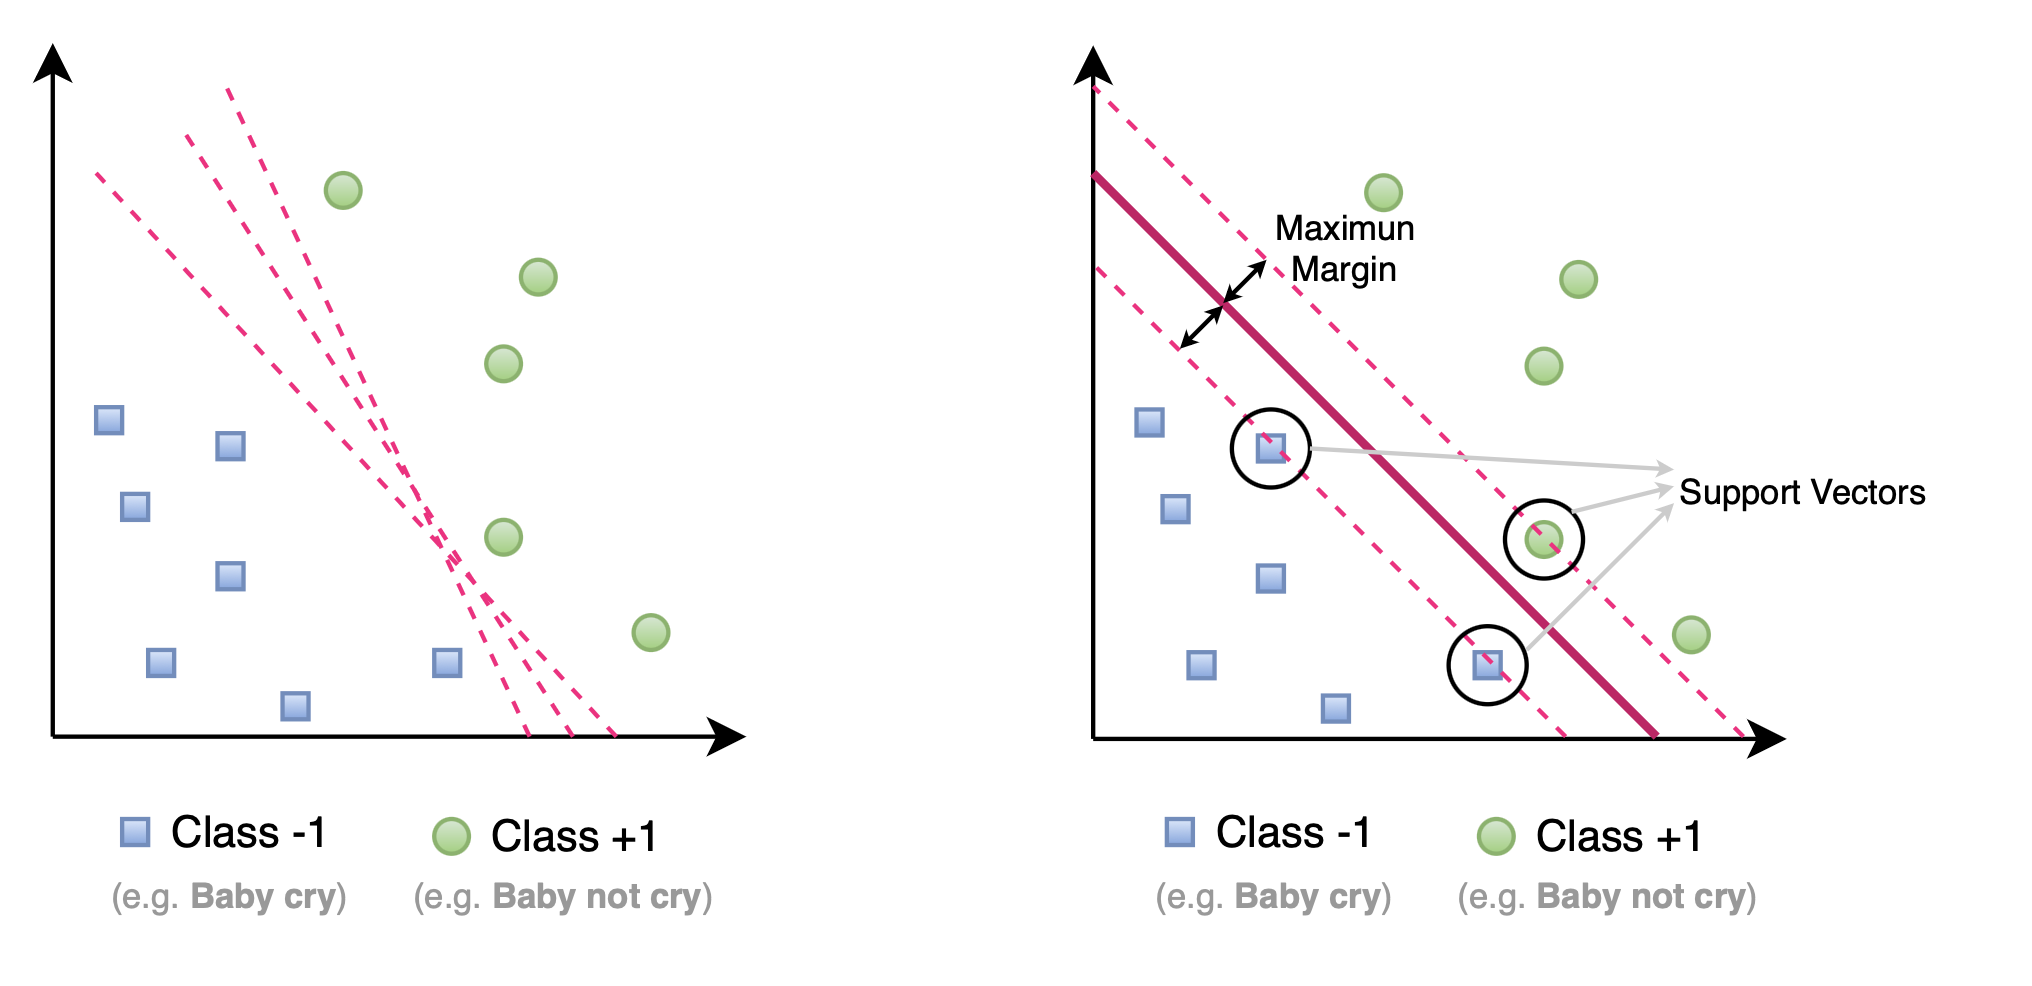
\includegraphics[width=0.9\textwidth]{figures/SVM-model.png}
\caption{Diagram of the SVM model}
\label{fig:SVM-model}
\end{figure}

\newpage
{\fontsize{16pt}{16pt}\textcolor{gray}{\textbf{Multi-class SVMs}}}

Although support vector machines are designed for solving binary problems, it is true that they can be applied to problems containing multi-class classifications \cite{Liao2019}. In order to apply SVM on multi-class classification problems, the dataset is divided into multiple binary classifications. These new subsets are then used to train the binary classification model (SVM). Using this approach, \textbf{One-vs-One (OvO)} and \textbf{One-vs-Rest (OvR)} strategies can be implemented. 

\vspace{\baselineskip}
Firstly, \textbf{One-vs-One (OvO)}, has the particularity of making pairs with the available classes, creating a data set of two classes in which one is the positive class and the other is the negative class, in this way, if there are K classes, \( \frac{k(k-1)}{2} \) different classifiers will be trained, as can be seen in the image \ref{fig:OvO-SVM-model}. As indeed may be observed, the number of classifiers grows quadratically with the number of classes, this aspect can make the model computationally expensive in terms of time and memory, especially with a large number of classes.

\textbf{One-vs-One (OvO) is the default for non-linear kernels.}

\begin{figure}[h]
\centering
    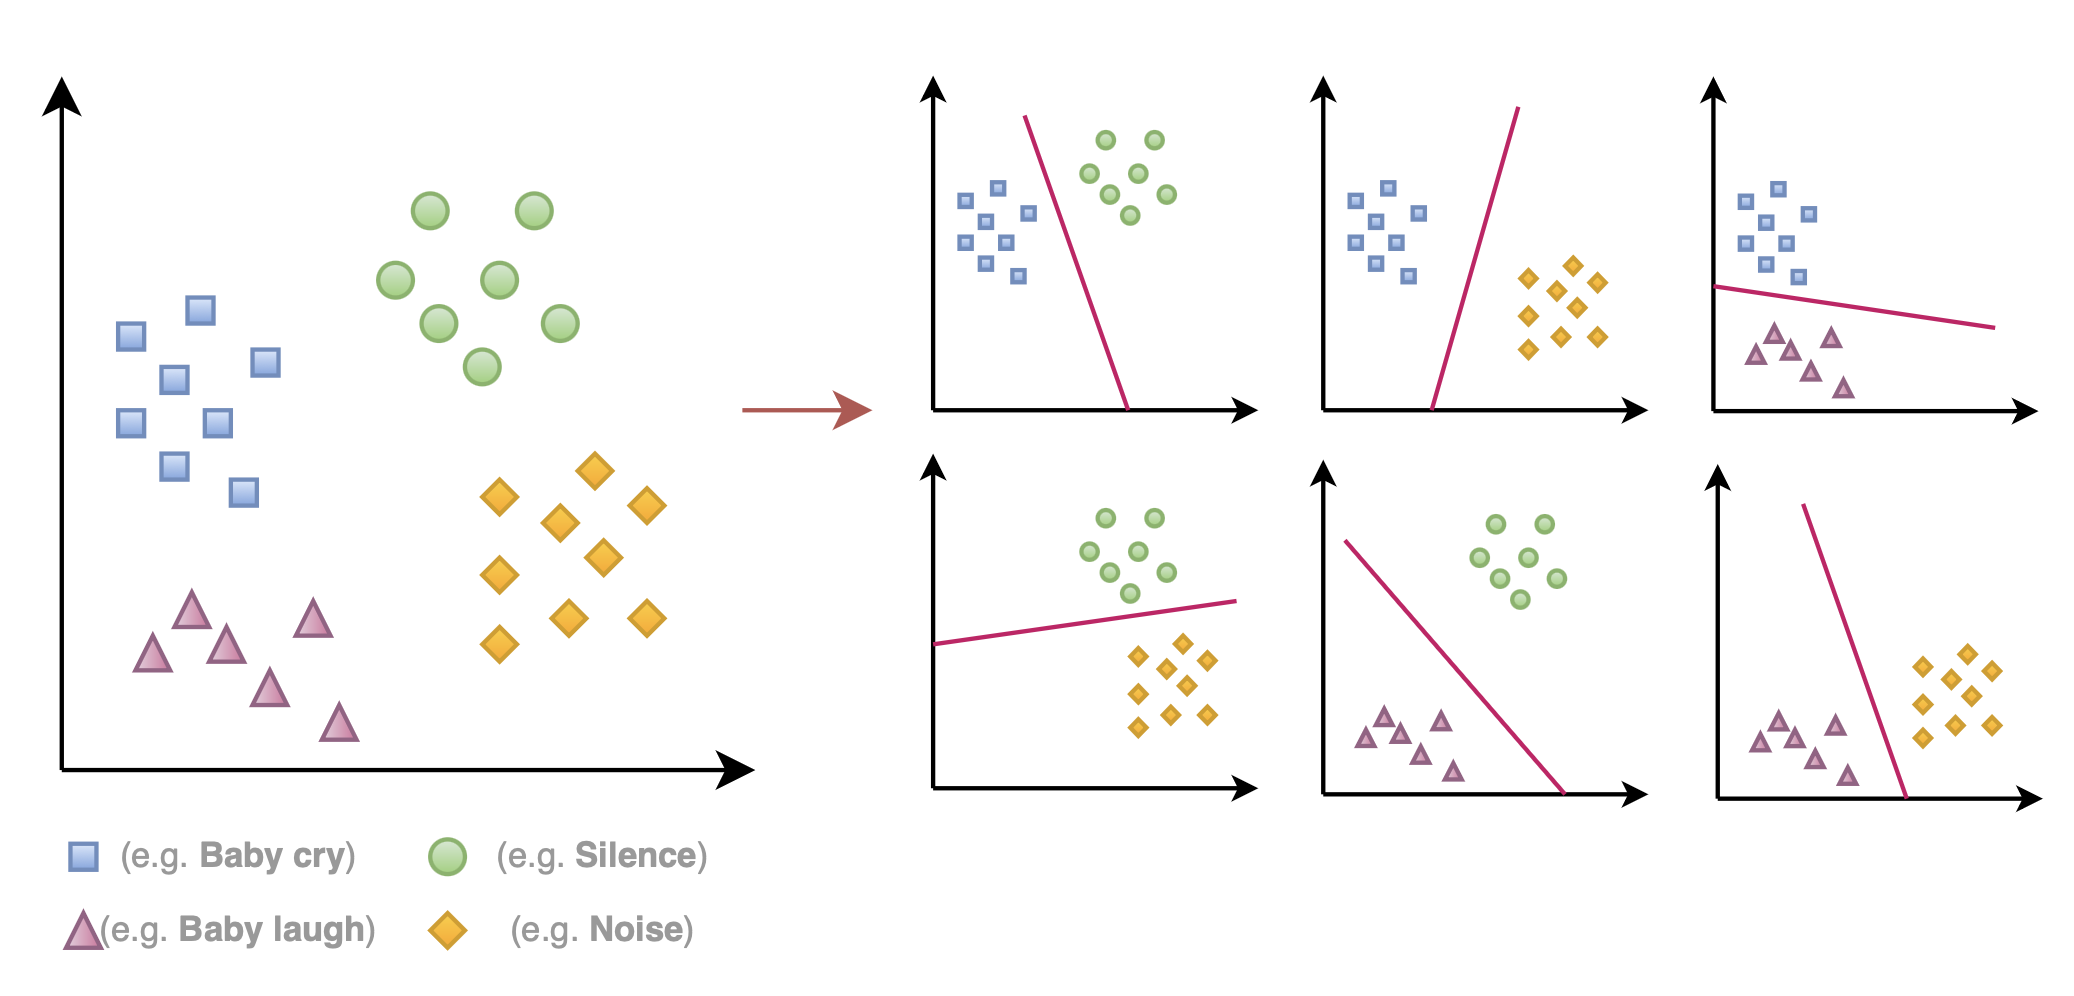
\includegraphics[width=1\textwidth]{figures/One-vs-One.png}
\caption{Diagram of the One-vs-One}
\label{fig:OvO-SVM-model}
\end{figure}

\vspace{\baselineskip}
Secondly, \textbf{One-vs-Rest (OvR)} again generates different binary classifiers to solve multi-class classification tasks. In this case, an SVM is trained for each class against the rest of the classes combined. That is, if there are a total of K classes, a total of K classifiers will be created, as can be seen in the image \ref{fig:OvR-SVM-model}. For each class k, an SVM classifier is trained to assigns the examples of class k as positive and the rest of the classes as negative. The prediction is performed as follows: first, each of the k binary classifiers evaluates the test example (or instance). Then, the class whose classifier returns the highest value of the decision function is selected. This class is considered the most likely class for the observation according to the model.


\textbf{One-vs-Rest (OvR) is the default value for linear kernels.}

\begin{figure}[h]
\centering
    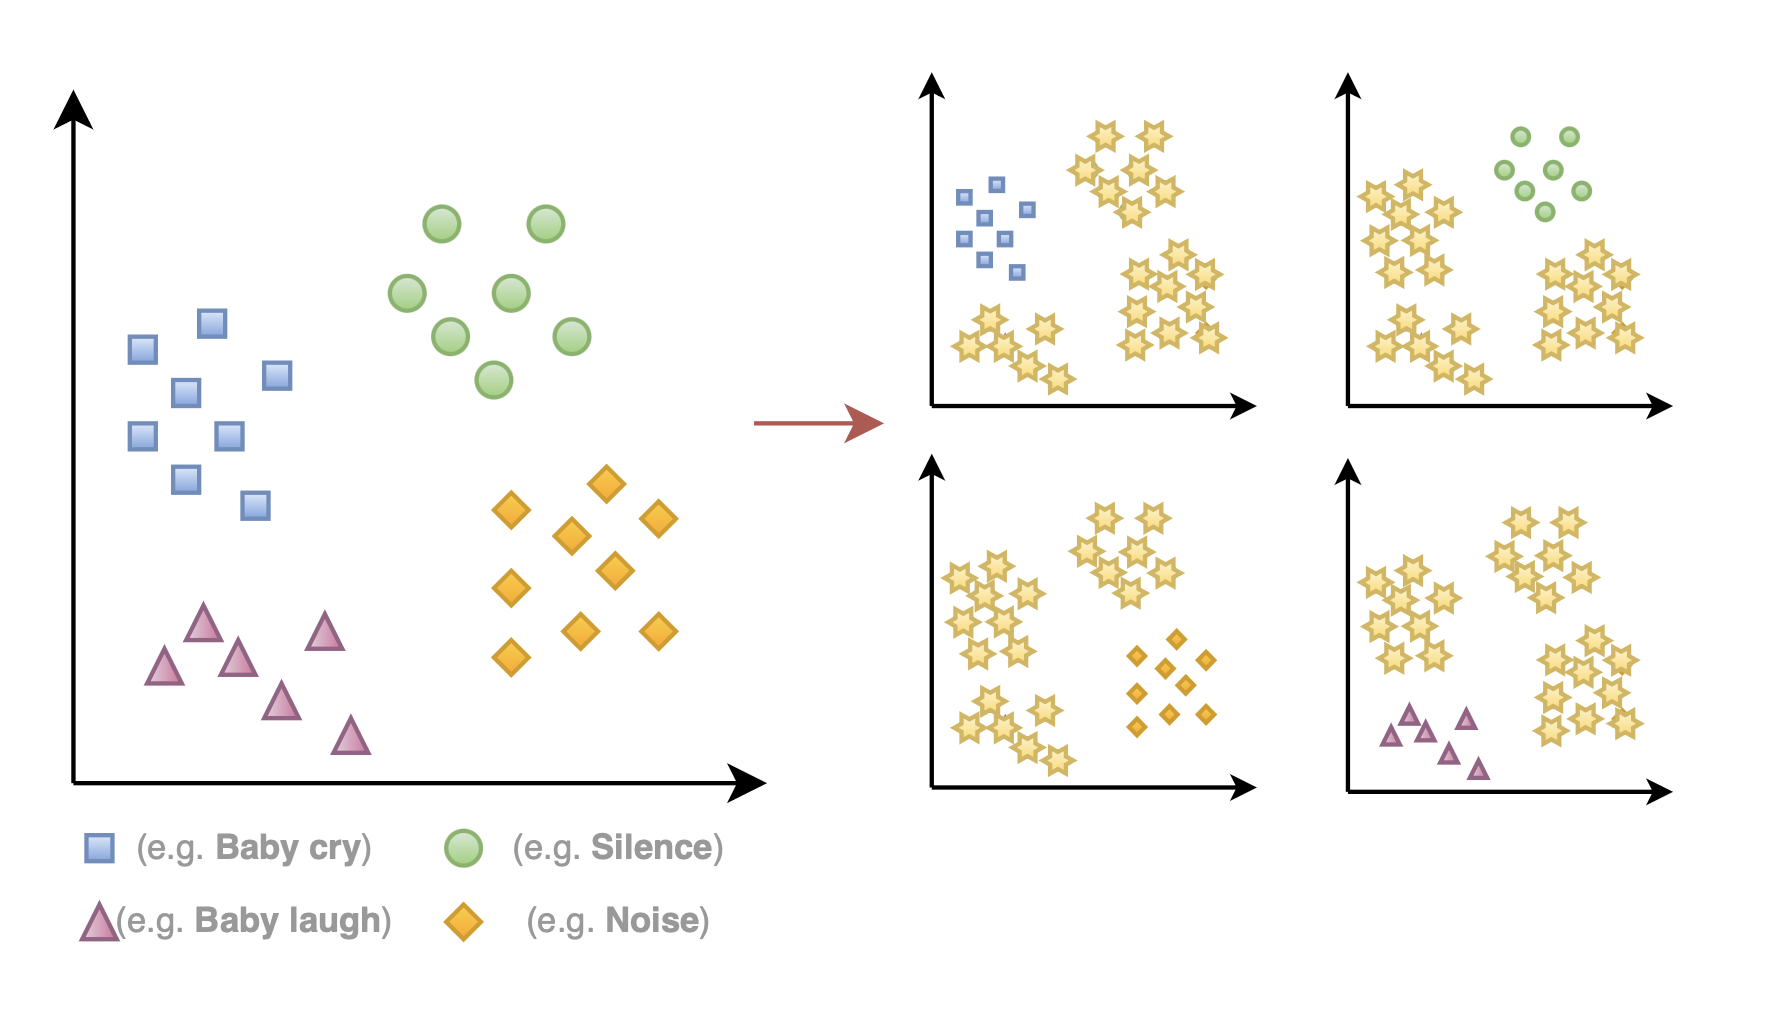
\includegraphics[width=1\textwidth]{figures/One-vs-Rest.png}
\caption{Diagram of the One-vs-Rest}
\label{fig:OvR-SVM-model}
\end{figure}

\newpage

{\fontsize{16pt}{16pt}\textcolor{gray}{\textbf{SVM implementation}}}

As with MLP, the \textbf{Scikit-learn} Python library has also been used to develop the model. The SVC (Support Vector Classification) class has been used for this purpose, as it allows the use of different kernel types and the possibility of calibrating the probabilities in the output.


As has been seen in the literature review, some studies highlight the use of the RBF kernel for its ability to handle non-linear data, and its good performance in classification problems. In this study, as it has been observed in the feature extraction in the images \ref{fig:pca-tsne-umap} it can be seen how the data are not linearly separable, that is, they cannot be separated with a straight line. Therefore, by using the \textbf{RBF kernel}, the data is projected into a higher dimensional space where it is more likely to find a hyperplane that separates the classes. 

The control parameter C, controls the trade-off between maximising the margin or minimising the classification error. A high value such as \( C = 10 \) penalises classification errors more, forcing the model to fit the training data more accurately. However, a low heat such as \( C = 1 \) allows for a wider margin and tolerates more classification errors, which can also help with model generalisation. 

In addition, \textbf{probability=True} is used to obtain probabilities on the model outputs instead of mere labels. This configuration makes it possible to interpret the SVM predictions in a more intuitive way. Instead of a simple binary classification indicating whether the baby is crying or not, the probabilities give an output between 0 and 1. This output is important to gradually observe changes in the baby's behaviour and to see how the probability of the baby crying varies.


\subsection{Long Short-Term Memory (LSTM)}
A Long Short-Term Memory (\textbf{LSTM}) network is a type of recurrent neural network (RNN) designed for the purpose of modelling long-term dependencies on sequential data \cite{Sak2014}. The main purpose for which they were designed was to handle the vanishing gradient problem that occurs in traditional RNNs, in these networks error is backpropagated through their multiple layers causing important information to be lost in the process. 

LSTM units are able to remember relevant data within a sequence and store this information during different instants of time. This feature makes the memory managed by these networks both long and short term, addressing the limitation that RNNs suffer from. 

The architecture of each LSTM unit includes the following main components:
\begin{itemize}
    \item \textbf{Cell}, is in charge of remembering values at different time intervals while the function of the gates is to regulate the flow of information both outside and inside the cell. This makes it feasible to maintain and modify information over long periods of time. 
    \item \textbf{State of the cell}, at this point the information from the entry gate and the forgetting gate is combined, i.e. the new information is combined with the information from the previous stage as indicated by the activations of the gates. 
    \item \textbf{Entry gate}, selects the new information to be kept within the cell state. 
    \item \textbf{Forgetting gate}, chooses which parts of the information belonging to the previous cell will be deleted. 
    \item \textbf{Output gate}, selects the relevant information that the cell state will use as output.  
\end{itemize}

\begin{tcolorbox}
This architecture has been widely used in speech recognition tasks because these are able to maintain relevant information over long audio sequences, which makes them especially suitable for the classification of events such as the cry of a newborn. 
\end{tcolorbox}


{\fontsize{16pt}{16pt}\textcolor{gray}{\textbf{LSTM implementation}}}

The implementation that has been carried out in this project on the LSTM model has been done by using \textbf{TensorFlow} together with \textbf{Keras} in Python. This combination results in a seamless integration allowing the construction of deep, and customised models, combining multiple types of layers such as Dropout and Dense.

The model that has been developed in this project is composed of a sequential architecture with \textbf{two LSTM layers} and \textbf{two Dropout layers} in order to effectively handle the input data streams. The first \textbf{LSTM layer} is designed with \textbf{64 units} and is configured to return complete sequences, capturing long-term temporal dependencies of the input data. 

Afterwards, a \textbf{Dropout layer} with a \textbf{rate of 0.5} is then applied, allowing a percentage of units from the previous layer to be disabled in order to help prevent overfitting during training. Then, the second \textbf{LSTM layer} is designed, this time with \textbf{32 units}, summarising the information from the previously processed sequences and returning a single output vector. This layer is also followed by a \textbf{Dropout layer} with a \textbf{rate of 0.3}, adding additional robustness to the model.

Finally, the model ends with a \textbf{Dense layer} with a \textbf{sigmoid activation}, adapted for a binary classification problem. The choice of sigmoid activation allows the model output to be interpreted as a probability between 0 and 1, which is especially useful for model evaluation using metrics such as the ROC curve and for decision making based on probabilistic thresholds. 


\section{Evaluate models}

To evaluate the performance of the Machine Learning and Deep Learning models, presented in the previous section, it is essential to use \textbf{quantitative metrics}. These metrics allow an objective and accurate assessment of the true performance of the models by providing concrete numerical values that facilitate the understanding of the models' performance. 

In this context of classification model evaluation, it is essential to keep in mind the following concepts that form the basis of many other metrics that will be discussed below: 
\begin{itemize}
    \item True Positives (\textbf{TP}), are the cases where the model correctly predicts the positive class, i.e. both the predicted value and the true value are positive. 
    \item False Positives (\textbf{FP}), are the cases where the model incorrectly predicts the positive class, predicting a class as positive when its actual value is negative. 
    \item True Negatives (\textbf{TN}), are the cases where the model correctly predicts the negative class, i.e. both the predicted value and the true value are negative. 
    \item False Negatives (\textbf{FN}), are the cases where the model incorrectly predicts the negative class, predicting a class as negative when its actual value is positive.
\end{itemize}

These four definitions above provide the support for creating various quantitative metrics. 
The precision metrics used in this project are defined below and are also summarised in the image \ref{fig:quantitative}: 
\begin{itemize}
    \item \textbf{Precision}, this value measures how well or poorly the positive predictions of the model have been realised. This is done by calculating the proportion of true positives out of the total number of predicted positive values.
    \item \textbf{Recall}, this value identifies how accurately the positive instances of the model have been classified. This is done by calculating the proportion of true positives over the total number of true positives.
    \item \textbf{F1-score}, this value is the harmonic mean between the recall and precision values. 
    \item \textbf{Accuracy}, this value expresses the proportion of correct predictions out of the total number of predictions made. This metric is useful to get a general idea of the model's performance, but be aware that this result may not be sufficiently accurate. In unbalanced ensembles this value may give a result close to one which would be interpreted as a good result, but this may be because it is conditioned by the predominant class. 
    \item \textbf{Confusion matrix}, this matrix clearly, and concisely represents the performance of the model. It shows a comparison between the predictions made by the model and the actual values. With this metric you can effectively compare whether the model's performance is being effective on unbalanced sets by looking at the percentage of data that is misclassified in each class. 
\end{itemize}

\begin{figure}[h]
\centering
    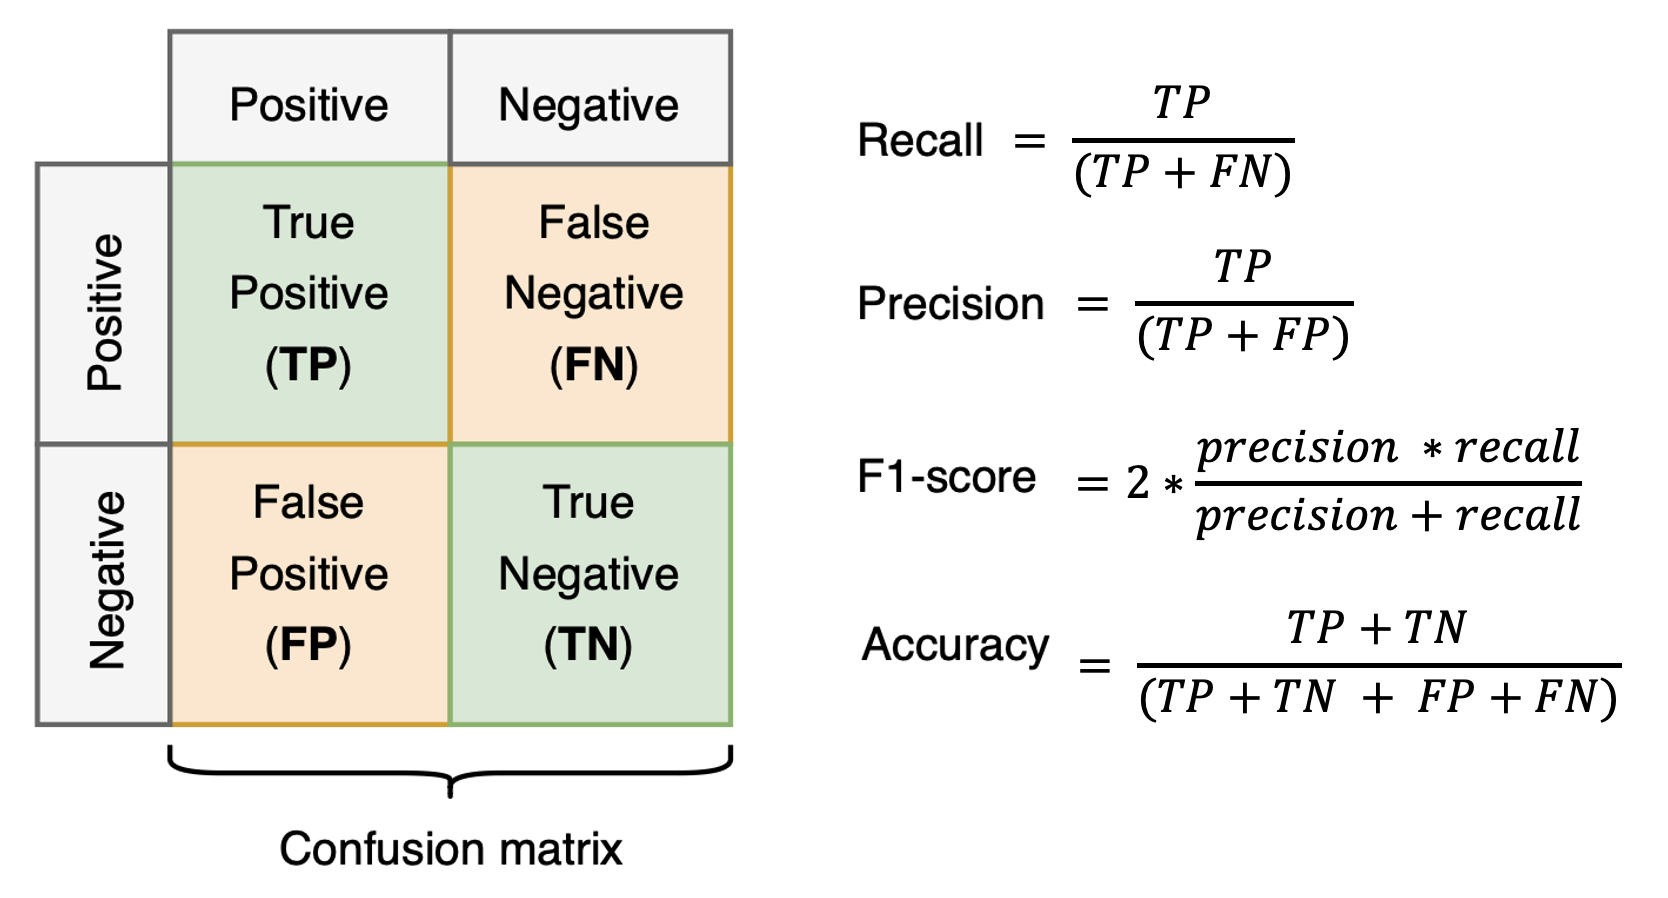
\includegraphics[width=0.5\textwidth]{figures/quantitative-metrics.png}
\caption{Summary of quantitative metrics}
\label{fig:quantitative}
\end{figure}

Nevertheless, the Receiver Operating Characteristic (\textbf{ROC}) curve, and the Area Under the Curve (\textbf{AUC}), are metrics that allow the performance of the model to be evaluated across different classification thresholds. 

The \textbf{ROC} curve is constructed from the true positive rate (\textbf{TPR}) previously defined as recall versus the false positive rate (\textbf{FPR}). This representation is generated together with a representation of a random classifier, where in the generated graph what would correspond to the Y-axis are the TPRs and what would correspond to the X-axis are the FPRs, as can be seen in the image \ref{fig:ROC}. The result is interpreted by observing how close the generated curve is to the perfect classifier. 

On the other hand, the \textbf{AUC} value summarises the information from the ROC curve into a single metric, i.e. a numerical value. For a perfect classifier this value would be equal to one, so the closer the result is to this value, the better the model is classifying. 

\begin{figure}[h]
\centering
    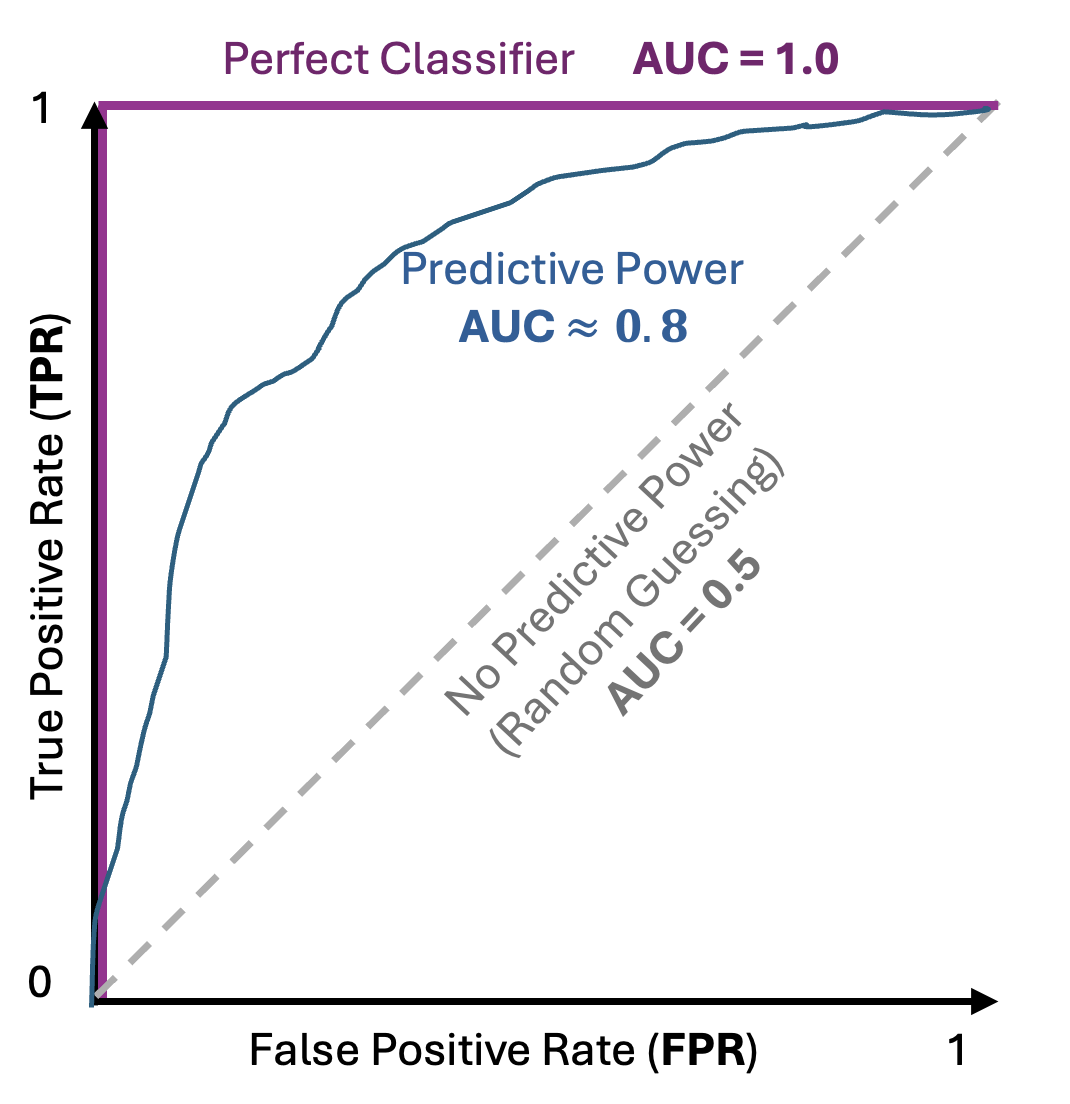
\includegraphics[width=0.4\textwidth]{figures/ROC-curve.png}
\caption{Functioning of the ROC Curve}
\label{fig:ROC}
\end{figure}


\section{Experiments}

Aforementioned, we want to compare the rankings offered by Machine Learning and Deep Learning models in order to obtain the best one. In addition we want to compare other factors of interest: analysis of feature extraction techniques (\textbf{MFCC}, \textbf{LPC}), the consequences of applying \textbf{cross-validation} on the models (\textbf{MLP}, \textbf{SVM}, \textbf{LSTM}), the effects of L2 regularisation, the use of different kernel types in SVM and possible layer configurations in LSTM. Consequently, we start with experiments using an already labelled dataset (multi-class classification) due to its high quality. These data clearly represent different types of sound, including baby cries, which makes them perfect for our purpose. The clarity and accuracy of these data are ideal for testing our models, ensuring that they work well and providing a solid basis on which to build the real project data (binary classification). 

\subsection{Multi-class classification}

To start with simple experiments that beforehand were expected to obtain good results, we used a dataset available on \myurl{https://github.com/giulbia/baby_cry_detection.git}{GitHub} characterised by the clarity with which it represents the different sounds, including the plain one. All the experiments performed with this dataset are summarised in the table \ref{table:multi-class-experiments}.

First of all, several experiments have been performed using Multilayer Perceptron (\textbf{MLP}) both "with", and "without" cross-validation. To perform these tests, we started by training a \textbf{MLP without cross-validation} with \textbf{300 hidden units}, dividing the dataset into 70\% for the training part and allocating 30\% of the remaining data for the test part. To perform this splitting process a random seed has been used to make this process consistent each time the code is run, ensuring that the training, and test sets are consistent across different runs. This \textbf{random seed} has been defined with a value equal to forty-two (42). In addition, the data has been standardised using \textit{StandardScaler} to have a mean of 0, and a standard deviation of 1, allowing for better efficiency, and stability in training the models. This ensures that all features contribute equally to the model predictions.

Afterwards, a stratified \textbf{five-fold cross-validation} has been implemented in order to split the data into multiple training, and test subsets. During each iteration of the cross-validation, features have been scaled, and the model has been trained and evaluated with the corresponding test subset. In addition, all actual labels and predictions in each of the folds have been accumulated. This accumulation makes it possible to subsequently calculate evaluation metrics such as the confusion matrix, and classification reports. 

These experiments are summarised in the notebook \myurl{https://github.com/lnc1002/TFM-Newborn_Cries_Classification/blob/4d0c85c8b15c2c117ca147f7c9625d47ff986ad8/src/2)\%20Second_steps/4_Notebook-4_MLP_Multi-class.ipynb}{2)Second\_steps/4\_Notebook-4\_MLP\_Multi-class.ipynb} .

Secondly, a larger number of experiments have been conducted using the Support Vector Machine (\textbf{SVM}) both "with", and "without" cross-validation. In this case, the experiments were also carried out with different classification strategies (One-vs-Rest and One-vs-One). On this occasion, the steps followed are the same as those described for the MLP model without cross-validation, except that in this case, a classification function (OvO or OvR) is applied before training the model. That is, for each feature extraction technique (MFCC and LPC) two different SVM models have been trained and evaluated, OvR training one classifier for each class and OvO training one classifier for each pair of classes.

Then, a \textbf{five-fold stratified cross-validation} has been implemented using a processing pipeline that includes: feature scaling, feature selection, and dimensionality reduction (PCA). Feature selection selects the best features based on the test score and \textbf{PCA} produces a set of \textbf{10 principal components}. With this new dataset as much variance as possible is preserved, making the model concentrate on the most informative features. This not only simplifies the model and speeds up the training process, but can also improve the generalisability of the model by reducing the risk of overfitting. 

These experiments are summarised in the notebook \myurl{https://github.com/lnc1002/TFM-Newborn_Cries_Classification/blob/4d0c85c8b15c2c117ca147f7c9625d47ff986ad8/src/2)\%20Second_steps/5_Notebook-5_SVM_Multi-class.ipynb}{2)Second\_steps/5\_Notebook-5\_SVM\_Multi-class.ipynb}.

Thirdly, the last experiments have been performed with Long Short-Term Memory (\textbf{LSTM}) and again "with", and "without" cross-validation. For the experiments without cross-validation, data splits of 70\% for training and 30\% for testing have been created with a \textbf{random seed} of value forty-two (42). Then, taking into account that a multi-class classification problem is being handled, a very important step is that the \textbf{labels} have been converted to the \textbf{one-hot} format. This model, when using the loss function \textit{categorical\_crossentropy} it is mandatory to convert the labels to one-hot in order to correctly calculate the loss and update the weights of the model. The last step during training, callbacks such as \textit{EarlyStopping} and \textit{ReduceLROnPlateau} were used to dynamically adjust the learning rate and prevent overfitting. \textit{EarlyStopping} monitors the loss in the validation set and stops training if there is no improvement after a specified number of epochs (\textit{patience}), thus preventing overfitting. \textit{ReduceLROnPlateau} reduces the learning rate if the loss in the validation set stagnates, allowing the model to find a global minimum more efficiently.

Finally, the LSTM neural network was used with a \textbf{five-fold stratified cross-validation} to robustly evaluate the model's performance. In this case the model setup is the same as in the previous case except that it is now trained, and evaluated many times on different subsets of the data. These tests, as in the previous models, are performed using both MFCC and LPC.

These experiments are summarised in the notebook \myurl{https://github.com/lnc1002/TFM-Newborn_Cries_Classification/blob/4d0c85c8b15c2c117ca147f7c9625d47ff986ad8/src/2)\%20Second_steps/6_Notebook-6_LSTM_Multi-class.ipynb}{2)Second\_steps/6\_Notebook-6\_LSTM\_Multi-class.ipynb}

\renewcommand{\arraystretch}{1.5} % Ajusta este valor según tus necesidades
\setlength\extrarowheight{5pt} % Ajusta este valor según tus necesidades
\begin{table}[!ht]
    \small
    \setlength\extrarowheight{2pt} % for a bit of visual "breathing space"
    \rowcolors {2}{gray!15}{}
    \begin{tabularx}{\textwidth}{>{\centering\arraybackslash}m{1.5cm} >{\centering\arraybackslash}m{1.5cm} >{\centering\arraybackslash}m{4cm} >{\centering\arraybackslash}m{8cm}}
    \hline
    \rowcolor{orange!10}
    \centering \textbf{Model} & \centering \textbf{Features} & \centering \textbf{Cross-validation} & \centering \textbf{Techniques} \\
    \hline
    MLP & MFCC & no & MLPClassifier \\
    MLP & LPC & no & MLPClassifier \\
    MLP & MFCC & yes & StratifiedKFold (5 splits), MLPClassifier \\
    MLP & LPC & yes & StratifiedKFold (5 splits), MLPClassifier \\
    SVM & MFCC & no & OneVsRestClassifier, kernel=linear \\
    SVM & LPC & no & OneVsRestClassifier, kernel=linear \\
    SVM & MFCC & no & OneVsOneClassifier, kernel=rbf \\
    SVM & LPC & no & OneVsOneClassifier, kernel=rbf \\
    SVM & MFCC & yes & StratifiedKFold (5 splits), OneVsRestClassifier, kernel=linear \\
    SVM & LPC & yes & StratifiedKFold (5 splits), OneVsRestClassifier, kernel=linear \\
    SVM & MFCC & yes & StratifiedKFold (5 splits), OneVsOneClassifier, kernel=rbf \\
    SVM & LPC & yes & StratifiedKFold (5 splits), OneVsOneClassifier, kernel=rbf \\
    LSTM & MFCC & no & LSTM, Dropout \\
    LSTM & LPC & no & LSTM, Dropout \\
    LSTM & MFCC & yes & StratifiedKFold (5 splits), LSTM, Dropout \\
    LSTM & LPC & yes & StratifiedKFold (5 splits), LSTM, Dropout \\
    \hline
    \end{tabularx}
    \vspace{10pt} 
    \caption{Summary of experiments on multi-class classification.}
    \label{table:multi-class-experiments}
\end{table}

\newpage

\subsection{Binary classification}

The experiments carried out with the data provided by the \textbf{HUBU} follow a similar approach to the previous experiments and are summarised in the table \ref{table:binary-experiments}, taking into account that in this case we are dealing with a binary classification. Furthermore, it is important to note that in this occasion the classes are \textbf{unbalanced} so the techniques modify the balance of the classes in the dataset, which is crucial in this context. Initially some experiments were carried out without balancing techniques, with the result that most of the correct predictions were concentrated in the majority class and more than 50\% of the minority class was misclassified. After observing these unfavourable results, the project focused its attention on experiments with balancing techniques such as \textbf{oversampling}, and \textbf{undersampling}. As these techniques are fundamental for handling class imbalance, the experiments that have been performed without them are not included in the project. 


First of all, experiments with the \textbf{MLP} model have been started for binary classification that follow a very similar approach to multiclass classification. Tests have been performed both "with", and "without" cross-validation, and both follow the same process. It starts with feature normalisation using \textit{StandardScaler}, and then combines oversampling, and undersampling using \textit{SMOTETomek} to address class imbalance. In addition, the classification threshold has been adjusted using the \textbf{ROC} curve to optimise the trade-off between true positive rate (TPR) and false positive rate (FPR). Again, these tests are performed using MFCC and LPC feature extraction techniques. 


These experiments are summarised in the notebook 
\myurl{https://github.com/lnc1002/TFM-Newborn_Cries_Classification/blob/4d0c85c8b15c2c117ca147f7c9625d47ff986ad8/src/3)\%20Final_steps/8_Notebook-8_MLP_Binary.ipynb}{3)Final\_steps/8\_Notebook-8\_MLP\_Binary.ipynb}.


Secondly, experiments have been followed by training and validating the \textbf{SVM} model with both MFCC and LPC feature extraction techniques. In addition, experiments "with", and "without" cross-validation have been carried out again, but this time the control parameter \( C \) has been modified by increasing its value in the tests with cross-validation. In the tests \textbf{without cross-validation} the value is \( C = 1 \) while in the tests \textbf{with cross-validation} the value is \( C = 10 \). This modification allows the model to fit the training data more closely, which is particularly beneficial to prevent overfitting. 

Moreover, the main steps have been kept intact in both experiments: feature normalisation, class balancing with \textit{SMOTETomek}, model calibration with \textit{CalibratedClassifierCV}, adjustment of the classification threshold using the ROC curve. 

These experiments are summarised in the notebook 
\myurl{https://github.com/lnc1002/TFM-Newborn_Cries_Classification/blob/4d0c85c8b15c2c117ca147f7c9625d47ff986ad8/src/3)\%20Final_steps/9_Notebook-9_SVM_Binary.ipynb}{3)Final\_steps/9\_Notebook-9\_SVM\_Binary.ipynb}

Thirdly, experiments with the \textbf{LSTM} model for binary classification have been completed, both "with", and "without" cross-validation, and by comparing the use of MFCC and LPC feature extraction techniques. In all experiments the same model structure is maintained with \textbf{two LSTM} layers and \textbf{two Dropout} layers using an output layer with \textit{sigmoid} activation instead of \textit{softmax}, and the loss function \textit{binary\_crossentropy}, being in this case a binary classification. Certainly, this time we have also used \textbf{oversampling} and \textbf{undersampling} techniques using \textit{SMOTETomek} to deal with class imbalance and scaled the features using \textit{StandardScaler}. 

Finally, in these \textbf{LSTM} experiments, techniques are used to improve the efficiency, and robustness of training in these deep neural networks. \textbf{EarlyStopping} reduces unnecessary training time in these deep models and \textbf{ModelCheckpoint} stores the most accurate, and generalisable version of the model, even if further training leads to a worsening of performance. These techniques show great utility in models such as LSTM due to their multi-layered structure, and the large number of parameters they possess, which translates into a high modelling capacity making them more susceptible to changes in the training data. This means that these models can learn complex patterns but also noise, which makes them more susceptible to changes in training data compared to simpler models such as MLP or SVM.


These experiments are summarised in the notebook \myurl{https://github.com/lnc1002/TFM-Newborn_Cries_Classification/blob/4d0c85c8b15c2c117ca147f7c9625d47ff986ad8/src/3)\%20Final_steps/10_Notebook-10_LSTM_Binary.ipynb}{3)Final\_steps/10\_Notebook-10\_LSTM\_Binary.ipynb}


\renewcommand{\arraystretch}{1.5} % Ajusta este valor según tus necesidades
\setlength\extrarowheight{5pt} % Ajusta este valor según tus necesidades
\begin{table}[!ht]
    \small
    \setlength\extrarowheight{2pt} % for a bit of visual "breathing space"
    \rowcolors {2}{gray!15}{}
    %\begin{tabularx}{\textwidth}{m{1.5cm}m{1.5cm}m{3.5cm}m{2cm}m{6cm}}
    \begin{tabularx}{\textwidth}{>{\centering\arraybackslash}m{1.5cm} >{\centering\arraybackslash}m{1.5cm} >{\centering\arraybackslash}m{3.5cm} >{\centering\arraybackslash}m{2cm} >{\centering\arraybackslash}m{6cm}}
    \toprule
        \rowcolor{orange!10}
        \textbf{Model} & \textbf{Features} & \textbf{Data Processing} & \textbf{Cross-validation}  & \textbf{Techniques} \\
    \midrule  
    MLP & MFCC & SMOTETomek, StandardScaler & no & MLPClassifier \\
    MLP & LPC & SMOTETomek, StandardScaler & no & MLPClassifier \\
    MLP & MFCC & SMOTETomek, StandardScaler & yes & StratifiedKFold (5 splits), MLPClassifier \\
    MLP & LPC & SMOTETomek, StandardScaler & yes & StratifiedKFold (5 splits), MLPClassifier \\
    SVM & MFCC & SMOTETomek, StandardScaler & no & SVC, CalibratedClassifierCV, kernel=rbf, C=1 \\
    SVM & LPC & SMOTETomek, StandardScaler & no &  SVC, CalibratedClassifierCV, kernel=rbf, C=1\\
    SVM & MFCC & SMOTETomek, StandardScaler & yes & StratifiedKFold (5 splits), SVC, CalibratedClassifierCV, kernel=rbf, C=10 \\
    SVM & LPC & SMOTETomek, StandardScaler & yes & StratifiedKFold (5 splits), SVC, CalibratedClassifierCV, kernel=rbf, C=10 \\
    LSTM & MFCC & SMOTETomek, StandardScaler & no & LSTM, Dropout \\
    LSTM & LPC & SMOTETomek, StandardScaler & no & LSTM, Dropout \\
    LSTM & MFCC & SMOTETomek, StandardScaler & yes & StratifiedKFold (5 splits), LSTM, Dropout \\
    LSTM & LPC & SMOTETomek, StandardScaler & yes & StratifiedKFold (5 splits), LSTM, Dropout \\
    \bottomrule
    \end{tabularx}
    \vspace{10pt} 
    \caption{Summary of experiments on binary classification.}
    \label{table:binary-experiments}
\end{table}


\newpage
\section{Results}
This section elaborates the results obtained from both the multi-class, and the binary classification of audio files. However, greater importance will be given to the results obtained in the \textbf{binary classification}, as this is the data provided by the HUBU, and is that which will enable the achievement of the project objectives. 

As mentioned above, to evaluate the performance of the models, different quantitative metrics have been used in the experiments, reserving qualitative metrics only for the binary experiments. These metrics express a more details on the effectiveness of the models, and are detailed in the experiment notebooks cited in the previous \textit{Experiment} section.


\subsection{Multi-class classification}

This section presents the results generated by the Machine Learning and Deep Learning models applied to the multi-class classification. As previously mentioned, this classification consists of four classes: \textbf{Crying\_baby (0), Silence (1), Noise (2), Baby\_laugh (3)}. The results of the different experiments are summarised in the table \ref{table:multiclass-results}. 

\renewcommand{\arraystretch}{1.5} % Ajusta este valor según tus necesidades
\setlength\extrarowheight{5pt} % Ajusta este valor según tus necesidades
\begin{table}[!ht]
    \small
    \setlength\extrarowheight{2pt} % for a bit of visual "breathing space"
    \rowcolors {2}{gray!15}{}
    \begin{tabularx}{\textwidth}{m{1.5cm}m{1.5cm}m{2cm}m{4.5cm}m{2cm}}
    \toprule
        \rowcolor{orange!10}
        \textbf{Model} & \textbf{Features} & \textbf{Cross-validation} & \textbf{F1-score (0, 1, 2, 3)}  & \textbf{Accuracy} \\
    \midrule  
    MLP & MFCC & No & 0.93, 0.97, 0.91, 1.00 & 0.95 \\
    MLP & LPC & No & 0.92, 1.00, 0.83, 1.00 & 0.95 \\
    MLP & MFCC & Yes & 0.93, 1.00, 0.93, 0.99 & 0.96 \\
    MLP & LPC & Yes & 0.89, 1.00, 0.87, 1.00 & 0.94 \\
    SVM & MFCC & No & 0.86, 0.98, 0.80, 1.00 & 0.92 \\
    SVM & MFCC & No & 0.88, 1.00, 0.73, 1.00 & 0.92 \\
    SVM & LPC & No & 0.98, 1.00, 0.96, 1.00 & 0.98 \\
    SVM & LPC & No & 0.90, 1.00, 0.77, 1.00 & 0.93 \\
    SVM & MFCC & Yes & 0.82, 0.97, 0.70, 0.96 & 0.87 \\
    SVM & MFCC & Yes & 0.84, 1.00, 0.80, 1.00 & 0.91 \\
    SVM & LPC & Yes & 0.93, 0.99, 0.91, 1.00 & 0.96 \\
    SVM & LPC & Yes & 0.88, 1.00, 0.85, 1.00 & 0.94 \\
    LSTM & MFCC & No & 0.84, 1.00, 0.76, 0.99 & 0.90 \\
    LSTM & LPC & No & 0.88, 1.00, 0.73, 1.00 & 0.92 \\
    LSTM & MFCC & Yes & 0.81, 1.00, 0.80, 0.97 & 0.90 \\
    LSTM & LPC & Yes & 0.83, 1.00, 0.73, 1.00 & 0.92 \\
    \bottomrule
    \end{tabularx}
    \vspace{10pt} 
    \caption{Summary of results on multi-class classification.}
    \label{table:multiclass-results}
\end{table}

The \textbf{MLP} model with MFCC features exhibits a good performance, and more stable results in the different classes, with an overall accuracy of 95\% without cross-validation, and slightly improves to 96\% with cross-validation. This model generates an adequate classification in the \textit{Crying\_baby} category, which is highly relevant to this project, and ensures proper detection of newborns’ cries. However, in this same model it can be observed how the LPC features show a slight decrease in the functioning of the \textit{Noise} category. This can cause various issues, such as detecting false positives in the detection or classification of crying.

On the other hand, the \textbf{SVM} model does not follow the same pattern as previously observed. In this model, the LPC features together with the OvO strategy that show the best results, especially without cross-validation, with an accuracy of 98\%. Additionally, as in the previous case, this model shows a slightly improved performance in the classification of \textit{Crying\_baby} however a better performance in the \textit{Noise} class stands out. Consequentially, the researcher can effectively distinguish between the cry of a baby, and the background noise, which has an astounding impact on our project. 

Finally, the \textbf{LSTM} model obtained very similar results when using MFCC features with, and without cross validation, with an accuracy of 90\%. Once more, the LPC features demonstrate a satisfactory performance with an accuracy of 92\%, and a consistency in the classifications of the \textit{Crying\_baby}, and \textit{Noise} classes.


\subsection{Binary classification}
This comprises of categorizing newborn audios into two classes that is \textit{Baby\_cry} and \textit{Baby\_not\_cry}. The results from this classification provide the real value in this project, as they focus on the detection of baby crying in a typical or representative setting. This data has been directly obtained from a hospital, so the \textit{Baby\_not\_cry} class comprises only environmental sounds typical in a hospital setting. The usage of this data ensures that the trained models are highly generalizable, and applicable in other health-related organizations, and similar environments.

This section describes the quantitative, and qualitative evaluation conducted in the binary classification including the pertinent metrics such as accuracy, and AUC, as well as a graphical representation of the probability of crying over time.

\vspace{\baselineskip}
{\fontsize{16pt}{16pt}\textcolor{gray}{\textbf{Quantitative experiments }}}

The results obtained in the binary classification are summarised in the table \ref{table:binary-results}. As seen in this table, all models show a higher capacity to detect the \textit{Baby\_not\_cry} class compared to the \textit{Baby\_cry} class. These results are as expected given the diversity of newborn cries in relation to amplitude, pitch, etc. It should be noted that accuracy in classifying the \textit{Baby\_not\_cry} class is critical to reduce false positives, while better classification of the \textit{Baby\_cry} class ensures a precise detection of crying.

Firstly, the \textbf{MLP} model with \textbf{MFCC} features shows strong results in both the “with”, and “without” cross-validation, notably the results obtained by the former, which generates an overall accuracy of 89\%. On this occasion, it can also be observed how the LPC features underperform, especially in the \textit{Baby\_cry} category, which could be problematic in the accurate detection of crying.

Secondly, in the \textbf{SVM} model it is observed both models “with” and “without” cross-validation present a solid performance, generating somewhat more accurate results in the experiments performed with \textbf{MFCC}, and the use of cross-validation. With this experiment, a remarkable accuracy is achieved in both classes, which can be seen in the F1-score values of 0.71 for the \textit{Baby\_cry} class, and 0.93 for the \textit{Baby\_not\_cry} class. By a very small margin, LPC is slightly less accurate than MFCC which could affect the system's ability to reliably detect crying. 


Finally, the \textbf{LSTM} model shows promising performance especially when the cross-validation technique is employed. The LPC features show an acceptable performance, although inferior to that of \textbf{MFCC}. With MFCC features, the model shows an F1-score of 0.70 for \textit{Baby\_cry}, and 0.93 for \textbf{Baby\_not\_cry} without cross-validation, with an accuracy of 0.89. However, the combination that best detects the \textit{Baby\_cry}, and the \textit{Baby\_not\_cry} class, is also by means of the MFCC features but this time with cross-validation, reaching an F1-score of 0.72, and 0.94 respectively, and an \textbf{accuracy of 90\%}, which was the highest in all conducted experiments. These findings suggest that LSTM models can be effective for the accurate detection of infant crying in hospital settings.


\begin{table}[!ht]
    \small
    \setlength\extrarowheight{2pt} % for a bit of visual "breathing space"
    \rowcolors {2}{gray!15}{}
    \begin{tabularx}{\textwidth}{m{1.5cm}m{1.5cm}m{2cm}m{2cm}m{2cm}m{2cm}}
    \toprule
        \rowcolor{orange!10}
        \textbf{Model} & \textbf{Features} & \textbf{Cross-validation} & \textbf{F1-score (0, 1)}  & \textbf{Accuracy} & \textbf{AUC} \\
    \midrule  
    MLP & MFCC & No & 0.69,    0.92 & 0.87 & 0.95 \\
    MLP & LPC & No & 0.62,    0.89 & 0.83 & 0.91 \\
    MLP & MFCC & Yes & 0.71,    0.93 & 0.89 & 0.95 \\
    MLP & LPC & Yes & 0.61,    0.90 & 0.84 & 0.91 \\
    SVM & MFCC & No & 0.67,    0.91 & 0.86 & 0.94 \\
    SVM & LPC & No & 0.61,    0.90 & 0.84 & 0.89 \\
    SVM & MFCC & Yes & 0.70,    0.93 & 0.88 & 0.94 \\
    SVM & LPC & Yes & 0.64,    0.92 & 0.87 & 0.90 \\
    LSTM & MFCC & No & 0.70,    0.93 & 0.89 & 0.95 \\
    LSTM & LPC & No & 0.64,    0.92 & 0.86 & 0.90 \\
    LSTM & MFCC & Yes & 0.72,    0.94 & 0.90 & 0.94 \\
    LSTM & LPC & Yes & 0.63,    0.92 & 0.86 & 0.90 \\
    \bottomrule
    \end{tabularx}
    \vspace{10pt} 
    \caption{Summary of results on binary classification.}
    \label{table:binary-results}
\end{table}

\newpage
{\fontsize{16pt}{16pt}\textcolor{gray}{\textbf{Qualitative  experiments }}}

The qualitative analysis focuses on visual assessment, so in this case different graphs reflecting the probability of crying over time have been generated. These results are based on the audio files that were not used in the previous experiments, and the directories are labeled as: \textit{Mild\_encephalopathy} (1 file), \textit{Severe\_encephalopathy} (1 file), \textit{Moderate\_encephalopathy} (1 file), and \textit{No\_encephalopathy} (2 files). To compare the results produced by the models, the graphs generated are going to be analyzed. In these graphs \ref{fig:cualitative-results}, a binary classification (0-1) can be observed where the probability of crying is either 100\% or 0\%. The precision or accuracy of the models can be determined if the pertinent graphs are somewhat similar to the first binary classification. This comparison identifies the nuances or other audio aspects thus offering a more representative understanding of the nature of the newborn cries. 


The models’ performance in identify audio cries from the new data provided improves slightly when using \textbf{MFCC features}, and applying \textbf{cross-validation}. For this reason, specific functions are used in this process that include the loading of the audio files, the extraction of MFCC features, the scaling of these features as required by the model, and the prediction of the probabilities for each class. Subsequently, the probabilities of crying per second in each audio file are plotted for a better visual understanding of the results. 

As can be seen in the images \ref{fig:cualitative-results}, \ref{fig:clips0-4}  all models predict crying quite well. In the case of \textit{Moderate\_encephalopathy} around the 18\textsuperscript{th} second a crying label is located but the models do not correctly detect the sound, in fact, the MLP model does not even detect crying at that moment. The rest of the models do detect something but with a probability of around 40\%. When the audio is played back to that time frame, a slight moaning cry is heard, so the models are not completely overlooking it. 

\begin{tcolorbox}
A snapshot of all the graphs identifies that the LSTM model performed slightly better than the other models in precisely predicting the probability of crying in the presented audios. 
\end{tcolorbox}
\vspace{\baselineskip}
\begin{tcolorbox}
\textit{The following images are composed of four graphs: the first (\textbf{blue}) shows the \textbf{label} graph, the second (\textbf{pink}) shows the prediction with \textbf{MLP}, the third (\textbf{green}) shows the prediction with \textbf{SVM}, the fourth (\textbf{orange}) shows the prediction with \textbf{LSTM}.}
\end{tcolorbox}

\begin{figure}[h]
\centering
    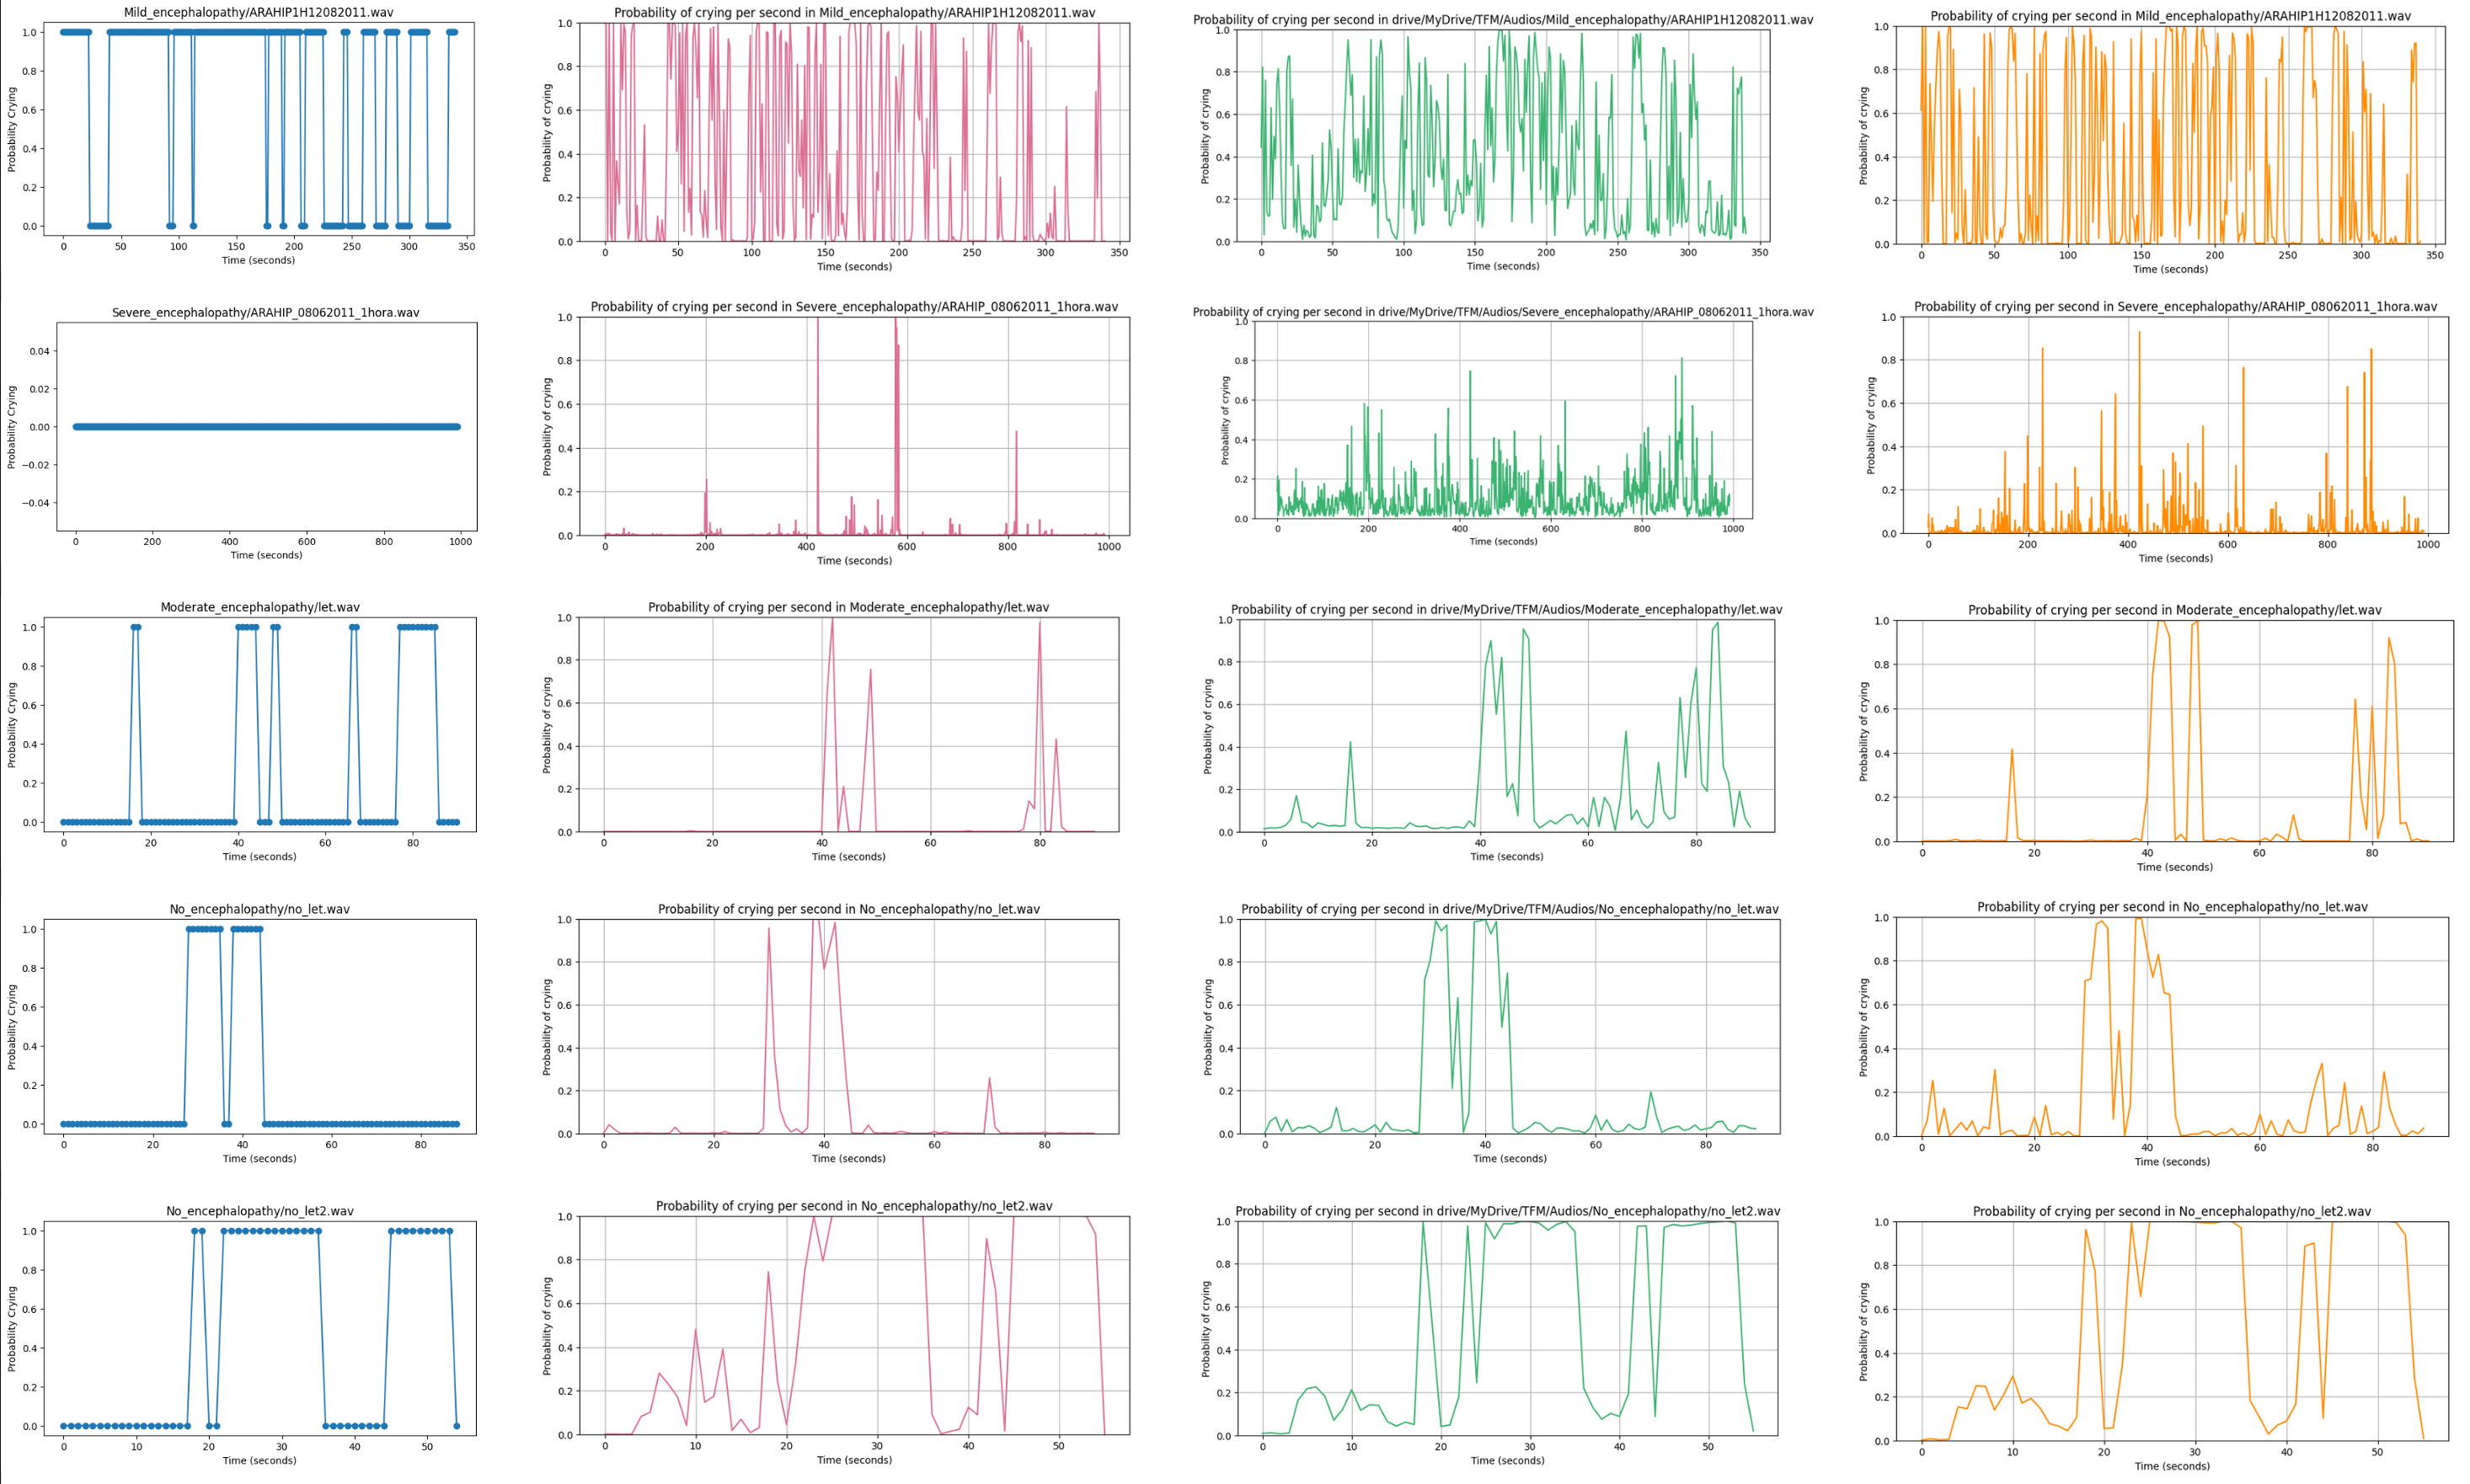
\includegraphics[width=0.85\textwidth]{figures/cualitative-results.png}
\caption{Predictions with different models \textit{a)} \textbf{blue} label graph textit{b)} \textbf{pink} prediction with MLP textit{c)} \textbf{green} prediction with SVM textit{d)} \textbf{orange} prediction with LSTM}
\label{fig:cualitative-results}
\end{figure}

\begin{figure}[h]
\centering
    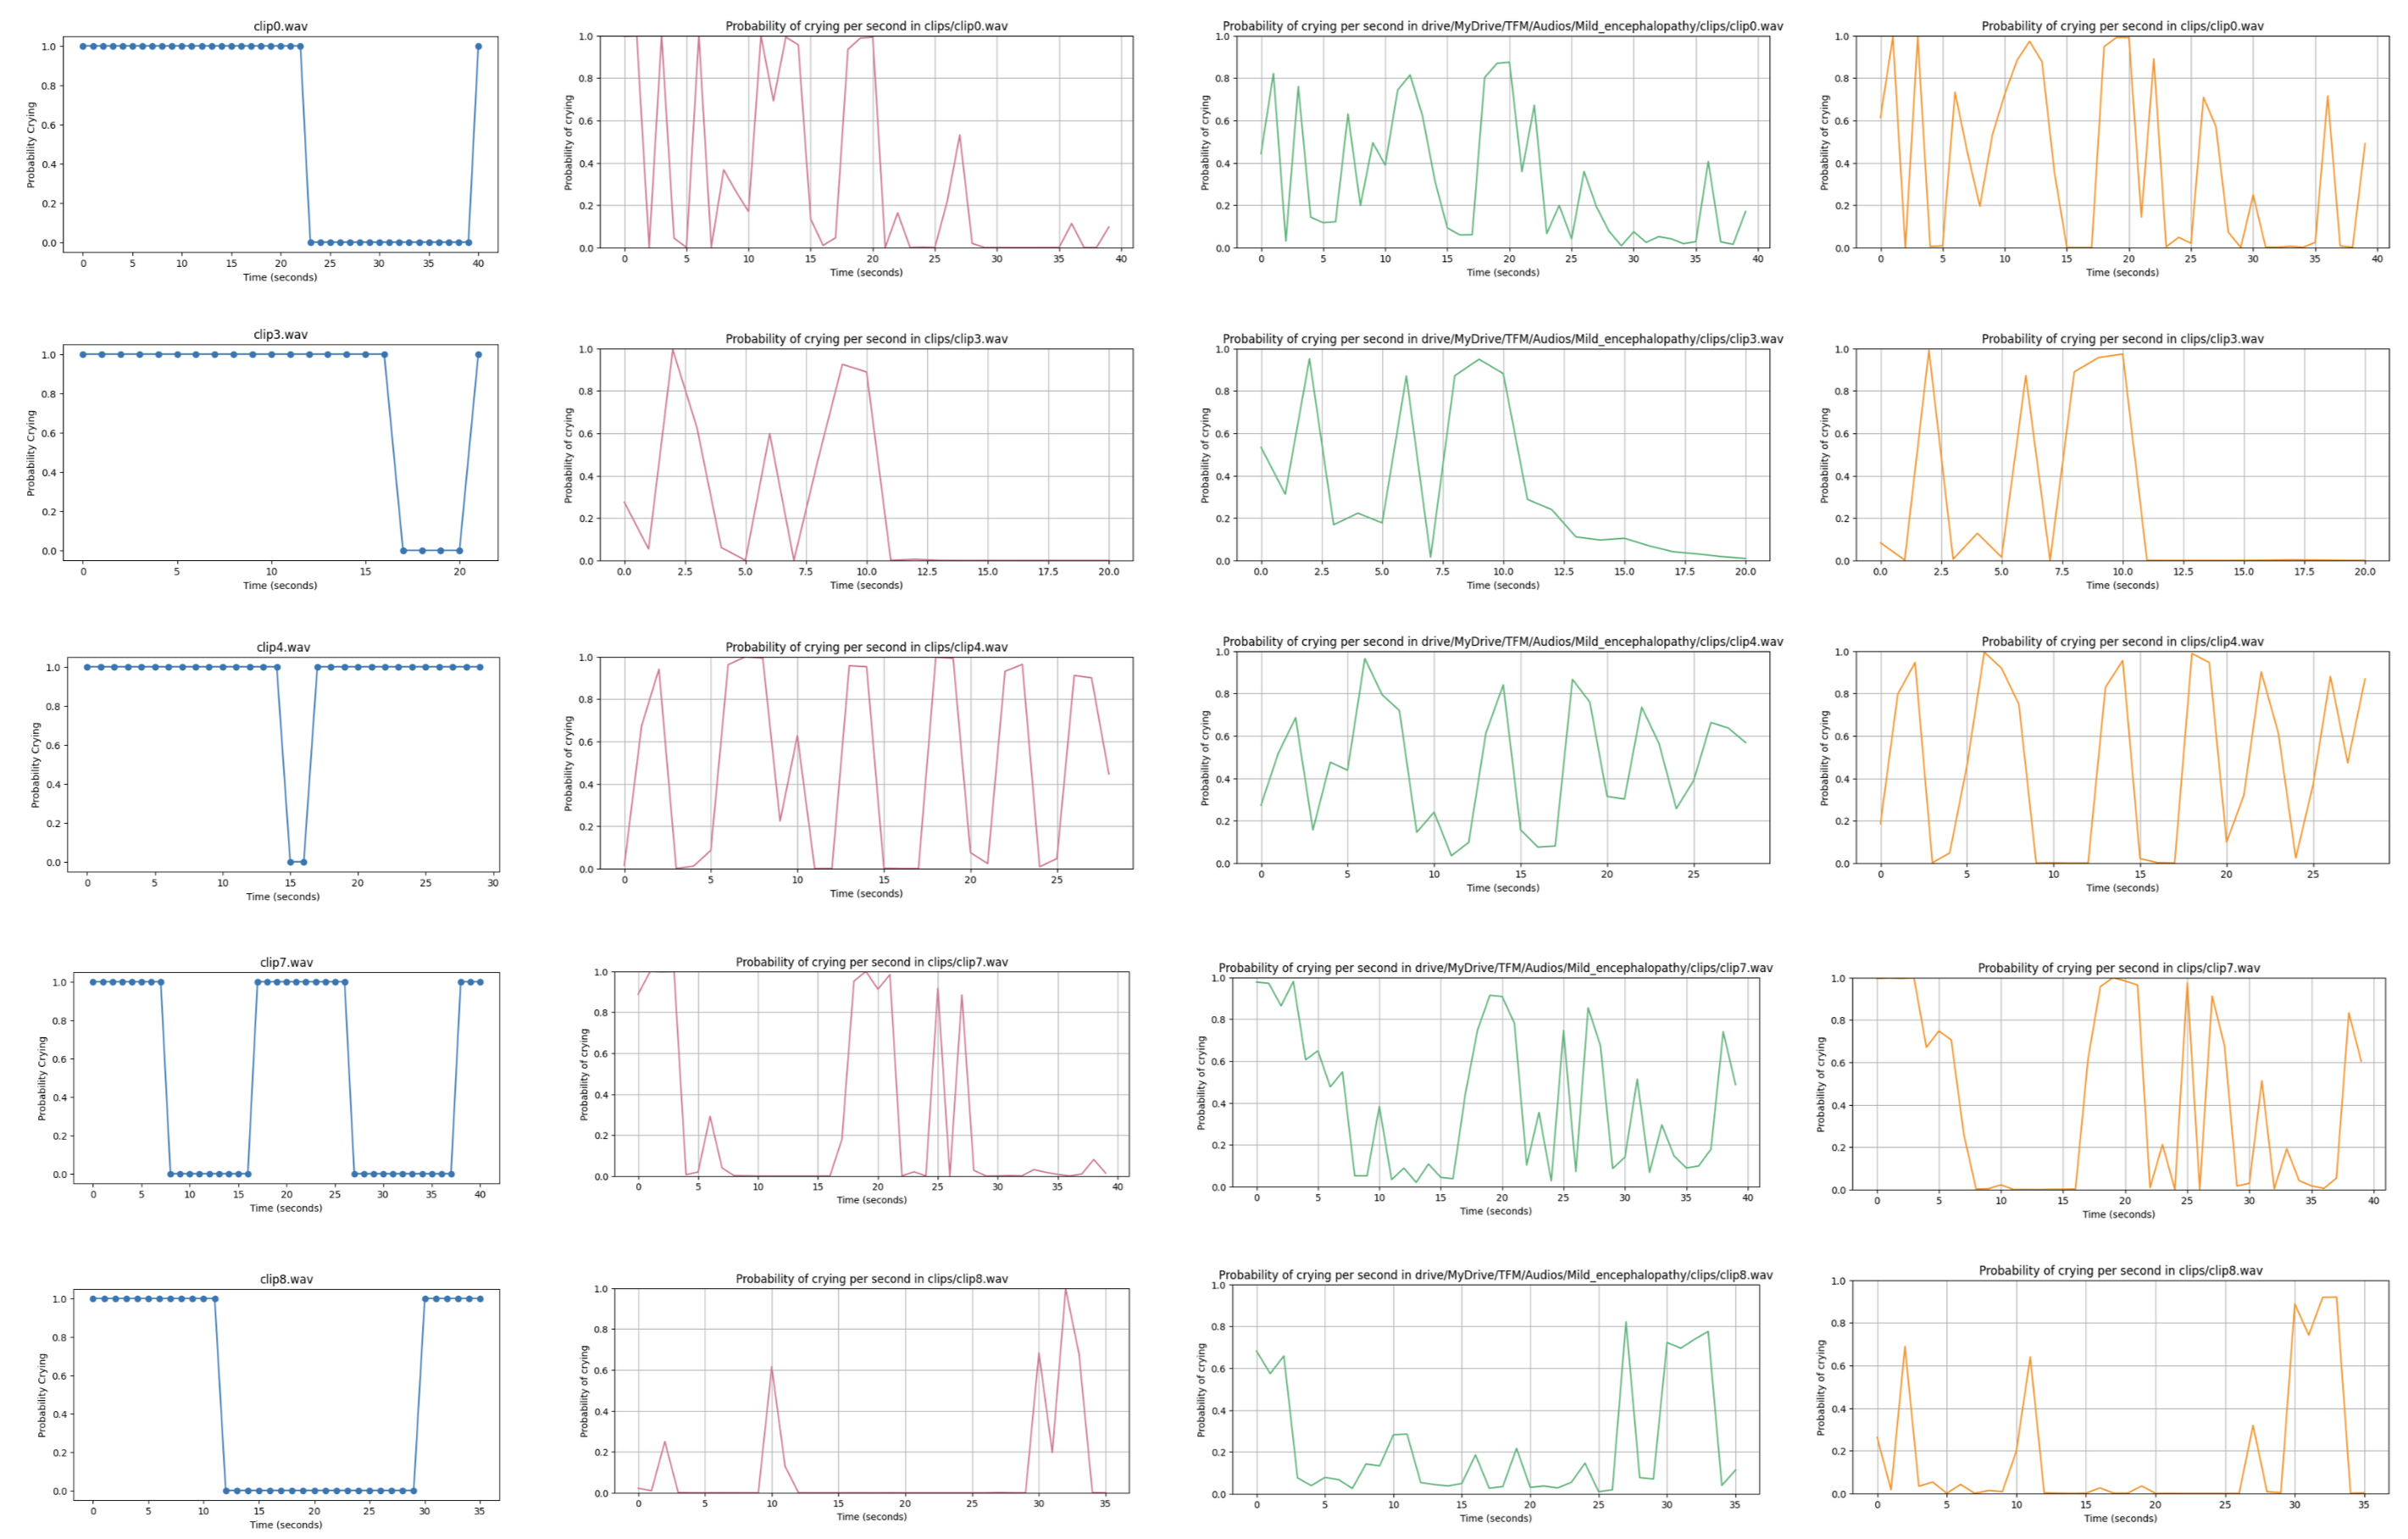
\includegraphics[width=0.85\textwidth]{figures/clips.png}
\caption{Predictions with different models in clips audio, \textit{a)} \textbf{blue} label graph textit{b)} \textbf{pink} prediction with MLP \textit{c)} \textbf{green} prediction with SVM \textit{d)} \textbf{orange} prediction with LSTM}
\label{fig:clips0-4}
\end{figure}
















